\synctex = 1

%%%% Copyright 2017 by Sean Luke
%%%% Distributed Under the Apache 2.0 License


\documentclass{article}
\usepackage{fullpage}
\usepackage{mathpazo}
\usepackage{microtype}
\usepackage{graphicx}
\usepackage{wrapfig}
\usepackage{amsmath}
\usepackage{amssymb}
\usepackage{array}
\usepackage{color}
\usepackage{rotating}
%\usepackage[nobottomtitles*]{titlesec}
\usepackage[noend]{algorithmic}
\usepackage{algorithm}
\usepackage{multicol}
\usepackage{ragged2e}
\usepackage[svgnames]{xcolor}
\usepackage[hyperfootnotes=false,linktocpage=true,linkbordercolor={0.5 0 0}]{hyperref}
\usepackage{tocloft}
\hypersetup{
    colorlinks,
    linkcolor={red!50!black},
    citecolor={blue!50!black},
    urlcolor={blue!80!black}
}%%% Note that to avoid a link being created from \pageref, just use \pageref*
%%% End hyperref stuff


\sloppy
\newcommand\ignore[1]{}
\newcommand\bump{\vspace{12in}}

\newcommand\myfrac[2]{#1/#2}
\begin{document}

\noindent {\Huge\bf Edisyn}\\[0.5em]
{\large \bf A Java-based Synthesizer Patch Editor and Librarian, Version 32\\[0.2em]
By Sean Luke\qquad sean@cs.gmu.edu}\\[0.2em]

\vspace{-1em}
\setcounter{tocdepth}{2}
%%% This is why we included tocloft.  See https://tex.stackexchange.com/questions/436063/spacing-between-number-and-text-in-toc
\advance\cftsecnumwidth 0.25em\relax
\advance\cftsubsecindent 0.25em\relax
\advance\cftsubsecnumwidth 0.25em\relax
\tableofcontents

\clearpage

%\vspace{0.5em}
\section{About Edisyn}

Edisyn is a no-nonsense synthesizer patch editor and librarian for the editing and parameter exploration of a wide variety of synthesizers.  It is not skeuomorphic or skinnable: its design is plain and consistent, though you can change the colors.  Edisyn is free open source.  Edisyn currently supports the following devices: 

{
\small
\begin{multicols}{2}
\begin{flushleft}
\begin{itemize}
%\item Futuresonus Parva
\item Alesis D4 and DM5 (Single)
\item Audiothingies MicroMonsta (Single)
\item Ashun Sound Machines Hydrasynth Family (Single)
\item Casio CZ-1, CZ-101, CZ-1000, CZ-3000, CZ-5000, and CZ-230S (Single)
\item Dave Smith Instruments Prophet '08 and '08 Desktop, Tetra, Mopho, Mopho Keyboard, Mopho SE, and Mopho X4 (Single and (for Tetra) Combo)
\item E-Mu Morpheus and Ultraproteus (Single, Hyperpreset, and MidiMap)
\item E-Mu Proteus 1, 1 XR, 2, 2 XR, 3, 3 XR, and 1+Orchestral (Single)
\item E-Mu Planet Phatt, Orbit and Orbit V2, Carnaval, Vintage Keys, and Vintage Keys Plus (Single)
\item E-Mu Proteus 1000/2000/2500, Audity 2000 v2.x, Virtuoso 2000, Xtreme Lead-1, Mo'Phatt, B-3, Planet Earth, Orbit-3, Proteus Custom, XL-1 Turbo, Turbo Phatt, Vintage Pro, XL-7, MP-7, PX-7, PK-6, XK-6, MK-6, Halo, and Vintage Keys Keyboard (Single)
\item Kawai K1, K1m, and K1r (Single and Multimode)
\item Kawai K4 and K4r (Single, Multimode, Drum, Effects)
\item Kawai K5 and K5m (Single and Multimode)
\item Korg SG Rack and SG Pro X (Single and (for SG Rack) Multimode)
\item Korg Microkorg (Single)
\item Korg Microsampler
\item Korg Volca Series: Bass, Beats, Drum, FM, Keys, Kick, NuBass, and Sample2 (Single); Drum (Split); Sample/Sample2 (Multimode), /u/pajen FM

\item Korg Wavestation SR (Performance, Patch, and Wave Sequence)
\item JL Cooper MSB Plus and MSB Plus Rev 2
\item M-Audio Venom (Single, Multimode, Arp, and Global)
\item Novation Drumstation and D Station
\item Novation SL, SL MKii, and SL Compact Series
\item Oberheim Matrix 6, 6R, and 1000 (Single and (for 1000) Global)
\item PreenFM2 (Single)
\item Red Sound DarkStar and DarkStar XP2 (Single and Per-Part)
\item Roland D-110 (Tone and Multimode)
\item Roland JV-80 and JV-880 (Single, Multimode, Drum)
\item Roland U-110 (Multi)
\item Roland U-20 and U-220 (Timbre, Multimode, Drum)
\item Sequential Prophet Rev2 (Single)
\item Waldorf Blofeld Desktop, Blofeld Desktop SL, and Blofeld Keyboard (Single and Multimode, plus wavetable uploading)
\item Waldorf Kyra (Single and Multimode)
\item Waldorf Microwave II, Microwave XT, and Microwave XTk (Single and Multimode)
\item Waldorf Pulse 2
\item Waldorf Rocket
\item Yamaha DX7 Family: DX7, TX7, TX216/TX816, Korg Volca FM, Dexed, DX200, DX9, etc. (Single)
\item Yamaha 4-Op FM Family: DX21, DX27, DX100, TX81Z, DX11, TQ5, YS100, YS200, B200, V50, etc. (Single and  (for TX81Z and DX11) Multimode)
\item Yamaha FB-01 (Single and Multimode)
\item Yamaha FS1R (Voice, Performance, and Fseq Modes)
\item Yamaha TG33, SY22, and SY35 (Single and (for TG33) Multimode)
\item General CC, NRPN, and RPN editing
\item Alternative tuning and Microtuning editing
\end{itemize}
\end{flushleft}
\end{multicols}
}

You'll note a pattern among these synthesizers: many are very difficult to program.\footnote{So why are the Prophet '08, Blofeld, Kyra, and Microwave XT there then?  Because these synthesizers are all ones I own or have had access to: that's another reason a synth might be in this list.  When I come into possession of an interesting synth, I build an editor for it.}  That's one of my interests.  

Edisyn's patch editors try to cover the most common needs, and so in most cases it does not support patches for global parameters, nor for wave, sample, or wavetable editing\footnote{The Blofeld patch editor only supports wavetable {\it uploading}, not {\it editing}: this is because there's an excellent free wavetable-editing tool available at https:/\!/synthtech.com/waveedit which is better than anything I could possibly write.} etc.  
%Additionally, though it can handle bulk downloads and files and manipulate them in a variety of ways, Edisyn is {\bf not at present a librarian tool}.  You should use a good free librarian software program, such as SysEx Librarian on the Mac.


\bump

\section{Starting Edisyn}
\label{startingedisyn}

\begin{wrapfigure}{r}{2.2in}
\vspace{-2em}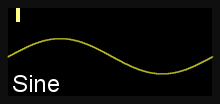
\includegraphics[scale=0.3]{0.png}
\vspace{-3em}\caption{Initial Synthesizer Dialog}\label{initialsynthpanel}
\end{wrapfigure}

If you're on a Mac, Edisyn will look like a standard application, just double-click on it.  On other platforms, Edisyn comes as a single Java jar file.  Just double-click on the jar file (you'll have to have Java installed) and Edisyn should launch.  See Edisyn's webpage for installation and launching instructions.

The first time you launch Edisyn, you'll be presented with the dialog at right, asking you to choose a synthesizer patch editor.  You can either select from {\it all} synthesizers available, or from those you have {\it recently} edited with Edisyn (the very most recent one is auto-selected for you). If you can't figure out why the {\it ``All Synths''} option is disabled, try first choosing ``{\it Select another synthesizer...}'' from the ``{\it Recent}'' popup.  

Once you've picked a synthesizer, if you click {\it Open}, Edisyn will attempt to connect to it via MIDI directly; you can also run in {\bf Disconnected Mode}, where you're not attached to MIDI.  And of course you can {\it Quit}.

\begin{wrapfigure}{r}{2.7in}
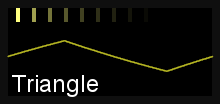
\includegraphics[scale=0.3]{1.png}
\vspace{-1em}\caption{MIDI Dialog}\label{mididialog}
\vspace{-3em}
\end{wrapfigure}

Edisyn will now build a patch editor for you and display it.  But unless you chose {\bf Disconnected Mode}, it'll first ask you to set up MIDI for this editor.  The dialog at right presents you with up to 6 fields (5 are shown here):

\begin{itemize}
\item The USB MIDI Device from which you will {\bf Receive} MIDI data sent by the synthesizer.  Here we are sending to a Tascam US-2x2 interface, which presents itself as a generic, nameless device. (BTW, if you're on a Mac and you don't like a generic name for your device, go to the Audio MIDI Setup application in the Utilities folder, double-click on the device, and change its name.)
\item The USB MIDI Device to which you will {\bf Send} MIDI to ultimately be sent to the synthesizer.  Here again we are sending to the Tascam US-2x2 device.
\item The {\bf Channel} on which the synthesizer is listening.  (Here, 1).
\end{itemize}

\vspace{-1em}
\vbox{
\begin{itemize}
\item (Not visible here) The optional {\bf ID} of the synthesizer.  Some synthesizers require a special ID embedded in their sysex so they can tell that the message is for them rather than another copy of the same synthesizer.  (The Yamaha TX81Z doesn't have an ID, so it's not displayed in this example).
\item The USB MIDI Device from which you will receive MIDI data sent by a {\bf controller}.  This may be a controller keyboard to play test notes on the synthesizer, or it may be a control surface to send CC data to the synthesizer or to Edisyn itself.  Here we are receiving from an Arturia Beatstep.
\item The {\bf Channel} over which you will receive MIDI data sent by a {\bf controller}.  This can be any specific MIDI channel, or (in this example) ``Any'', meaning any channel or OMNI.
\item The USB MIDI Device and MIDI Channel for a {\bf second controller}.  You can use this just like the first controller: you can drive the synthesizer or control Edisyn  from two different controllers at once.
\end{itemize}

If you are not connected to MIDI, or if you cancel, then Edisyn will inform you that you must continue in {\bf Disconnected Mode}.

\paragraph{Future Launches}  The next time you start up Edisyn, it won't show you the Initial Synthesizer Dialog.  Instead, it'll just pop up the last synthesizer editor type you had created.  If you'd prefer to see the Initial Synthesizer Dialog when launching, uncheck {\bf Launch with Last Editor} in the {\bf Options} menu.

%\paragraph{Important Note}  If your USB MIDI device is manually disconnected, Edisyn won't know until you ask Edisyn to send the synth something (perhaps changing a parameter or uploading a patch).  At that point, Edisyn will get a clue and the patch editor window will change to {\bf Disconnected Mode}.'
}

\section{Edisyn Patch Editors}

\paragraph{What exactly is a Patch?}  You probably think you know, but you might not.  From Edisyn's perspective, a {\bf patch} is something that Edisyn can store and retrieve on your synthesizer through MIDI commands; and usually there is a collection of patches each of which can be called up individually.  Some synthesizers (like the Yamaha DX7) are simple: they have 32 patches that you can upload and download and that's it.  Others are more complex: they may have {\it different kinds of patches}.  For example, many synthesizers have a set of patches which represent {\bf single sounds} and also a different set of {\bf multimode} patches which represent {\it multitimbral collections} of sounds defined by the single patches.  The multimode patches do not hold the single patches: they point to them.  Thus if you change a single patch, it's changed for every multimode patch which references it.  Some synthesizers might also have separate {\bf drum patches}, or {\bf effects patches}, etc.

Edisyn generally has one patch editor for each kind of patch in a synthesizer.\footnote{In some cases Edisyn doesn't implement an editor for a certain patch type.  Sometimes this is for patch types that are too arcane.  In other cases, certain patch types may not have adequate facilities to access easily via sysex: for example Korg Wavestation SR's multimode patches stupidly must {\it all} be uploaded and downloaded as a blob, rather than individually.  Edisyn also usually doesn't make editors for global parameters, except in certain rare cases.}

Most synthesizer manufacturers sensibly refer to their single patches as single patches and their multitimbral patches as multitimbral (or multimode) patches.  But other manufacturers\,---\,notably Roland\,---\,insist on a bizarre vocabulary for their different patch types.  For example, single patches on the Roland U-220 are called {\it timbres}, while the multimode patches are called {\it patches}, of all things.  This causes many Edisyn users to get confused, with questions such as ``Why does Edisyn say `upload patch' when it should say `upload timbre'?''  The answer is: Edisyn must be consistent in the face of some manufacturers' stupid naming decisions: every different patch type is always referred to as a {\bf patch}.

Other synthesizers (such as the Yamaha FS1R and the Roland D-110) try to hide the fact that they have different kinds of patches by pretending their single-mode and multimode patches are all one blob, presenting them to the user in a single convoluted unified interface, even if they're different patches over MIDI. This also confuses users, who wonder why Edisyn has multiple editors for a given synth.  But from Edisyn's perspective, they're separate patch types.  Edisyn will try to make it easy to navigate from one patch type to another through custom buttons or menu options as appropriate.

\begin{wrapfigure}{r}{3in}
\vspace{-2em}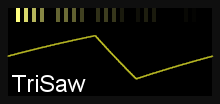
\includegraphics[scale=0.3]{2.png}
\vspace{-3em}\caption{Typical Patch Editor Panel (TX81Z)}\label{typicalpatcheditorpanel}
\vspace{-2em}
\end{wrapfigure}

\paragraph{Edisyn's Patch Editors.}  An Edisyn patch editor is a single window with multiple tabbed panes.  You can switch tabs by clicking on them or via shortcuts (see the {\bf Tabs Menu}).  The far-right tab is the {\bf About Tab}.  It gives you information about the eccentricities of the synthesizer that require custom behavior in Edisyn (they all do!).  {\bf \color{red} You should read the About Tab for your synth's editor \textit{carefully} to understand how to get Edisyn to work properly with your synthesizer.}

\definecolor{darkpastelgreen}{rgb}{0.01, 0.75, 0.24}
\definecolor{limegreen}{rgb}{0.2, 0.8, 0.2}
\definecolor{hanpurple}{rgb}{0.32, 0.09, 0.98}
\definecolor{mustard}{rgb}{1.0, 0.86, 0.35}
\definecolor{goldenyellow}{rgb}{1.0, 0.87, 0.0}
\definecolor{goldenrod}{rgb}{0.85, 0.65, 0.13}

\paragraph{Categories}
At right is a typical tab pane.  You'll note that various widgets are grouped together in regions (called {\bf Categories}).  There are four categories shown here.  Three are arbitrary categories for this synthesizer: ``{\bf {\color{limegreen}Global}}'', ``{\bf {\color{hanpurple}LFO}}'', and ``{\bf {\color{goldenrod}Controllers}}''.  They're in various colors to differentiate them.  Other categories will be found in other tab panes.  But one category is special: the {\bf Synthesizer Category}, always shown in white, here named ``Yamaha TX81Z''.  It normally contains the patch name and bank/patch number.

If you right-click, or Shift-click, on a category name, you'll get a pop-up menu with certain cut, paste, distribution, and reset options.  See Section~\ref{editing} for information about them.

\bump

\paragraph{Widgets}  Edisyn has a number of widgets.  Here are a few of them:

\begin{itemize} 

\item The {\bf Patch Display}, currently showing patch ``I004''.  Sometimes this display will be inaccurate, particularly if you manually change the patch on the synthesizer while Edisyn is running; or if Edisyn has no idea what the patch should be (it'll usually display a default value like, in this case, ``A001''.

\item The {\bf Patch Name Button}, currently showing ``DEMO SOUND''.  Click on this button to change the name of your patch.  A dialog will pop up to let you change the sound, with an additional {\bf Rules} button to explain the constraints the synthesizer places on patch names. Can't think of a name?  Press {\bf Rand} to generate a random \(4+\) letter word.

\item Displays of {\bf Keyboards}.  Select a key!
\end{itemize}

\begin{itemize}
\item Various {\bf Dials}. These are semicircles in gray, partly in some other color, with a value in the center.  Dials vary in orientation.  Most look sort of like a ``C'', with the zero point at the bottom center.  Other dials are symmetric, such as the ``Breath Ctrl. Pitch Bias'' dial (bottom row, second from right in the Figure), and have zero point at center top.  Occasionally dials have other orientations: the goal is to keep the zero point centered (at top or bottom).

You change values in a Dial by clicking on the dial and dragging vertically.  You can also double-click on a dial to reset it to a default value (often zero).  If the Dial doesn't have the finesse you require to hit an exact value, hold down the {\bf Alt} (or on the Mac, the {\bf Option} key while dragging and you'll get 4\(\times\) the resolution.  Hold down the {\bf Control} key and you'll get 16\(\times\) the resolution. Hold down both keys and you'll get 64\(\times\) the resolution!  Finally, you can  two-finger drag (on the Mac), or spin the mouse wheel to move the value by exactly 1 unit.  


\item {\bf Checkboxes} (such as ``Portamento'').  These are should be straightforward.

\item {\bf Pop-Up Choosers} or Combo Boxes (such as ``Wave'', set to ``Sawtooth'').  Ordinarily these work exactly as you expect.  However they have one surprise.  If you select the menu option {\bf Keep Next Popup Open} from the {\bf Options} menu, then the next time you click on a popup-chooser, its menu will stay open even after you have made a selection.  This allows you to try a variety of selections out without having to always reopen the popup menu.  This is particularly useful for large popups, such as for PCM wave samples.  You can get rid of the menu by clicking outside the menu or typing {\it Escape}.  

\item Various {\bf Pictorial Displays}.  Here, changing the ``Algorithm'' dial will modify the Algorithm Display immediately to the right of it.

\begin{figure}[t]
\begin{center}
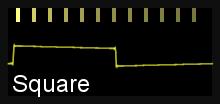
\includegraphics[scale=0.6]{4.png}
\end{center}
\caption{Envelope Displays of the Waldorf Microwave II, XT, and XTk.}
\label{envelopedisplays}
\end{figure}

\item Various {\bf Envelope Displays}.  Edisyn can draw envelopes using a variety of procedures.  Consider the Waldorf Microwave envelopes in Figure \ref{envelopedisplays} above, for example.  The first two envelopes are ADSR envelopes, but the third is the Microwave's famous ``Wave Envelope'', an eight-stage envelope with two different looping intervals (shown below it), and with two special end times marked with vertical lines (here, the dashed line is where optional sustain occurs, and the solid line is the end of the wave).    The last envelope is the Microwave's ``Free Envelope'', a four-stage envelope unusual in that it can have both positive and negative values: the dashed line is the axis.

Mose Edisyn envelope displays are read-only -- you can't draw the dots.  But that's not always the case: for example the Kawai K5 harmonics display can be extensively edited by mouse.

\item {\bf Action Buttons}.  Some patch editors have buttons on them which perform actions rather than edit or display values.  For example many multimode-patch editors have buttons that pop up single patch editors for the various individual patches.

\end{itemize}

If you are connected to a synthesizer over MIDI, then changing a widget will modify the underlying patch parameter in real time, if the synthesizer supports this.  Also, if you modify a parameter on the synthesizer, then Edisyn will update the corresponding widget or widgets (again, if the synthesizer supports this).

\paragraph{Changing Edisyn's Color Scheme}  If you find Edisyn ugly, you can change the colors with {\bf Change Color Scheme} in the {\bf Options} menu (or reset them with {\bf Reset Color Scheme}.  Note that not all widgets will change their colors until you have restarted Edisyn: until then, you'll get a weird mishmash of colors.

\section{Creating and Setting Up Additional Patch Editors}

A patch editor is created by selecting one of the various {\bf New...} menu options in the {\bf File} menu.\footnote{The {\bf New Synth} menu presents you with several options.  First there are the patch editors you have {\it recently selected}, if any.  Next come {\it all available} patch editors, organized by manufacturer.  Finally, you have menu choices to {\it remove} patch editors from the recent list.}   You have to create a new a patch editor before you can start loading a patch from a file or from the synthesizer.  You can also {\bf Duplicate} an existing patch editor (in the {\bf File} menu).  This will exactly duplicate the existing patch as well.  

Whenever you create a new patch editor or duplicate one, you will once again be asked to set up MIDI as discussed in Section \ref{startingedisyn}, or to run in Disconnected Mode.

\paragraph{Persistence}
Now would be a good time to mention an Edisyn feature you may never notice otherwise: many things are {\bf persistent}.  For example, if you choose ``Arturia Beatstep'' as the controller for your Blofeld patch, the next time you call up a Blofeld patch editor, ``Arturia Beatstep'' will be presented as the default choice in the MIDI Devices window, assuming your Arturia Beatstep is plugged in.  This goes for everything in the MIDI Devices window.  Furthermore, if you pop up a new patch editor for a synthesizer you have never edited before, the Arturia Beatstep will be the default option for that one too (until you change it one time).    And these options are per synthesizer type.

Persistence appears in other places too.  For example, the Initial Synthesizer dialog will default to the last synth you chose in that dialog.  Persistence shows up in many other places as well.

\paragraph{Selecting Patch Editor Windows} When you bring a patch editor window to the front, Edisyn sends a bunch of All Sounds Off MIDI messages to clean things up for the editor.  However this may sometimes be undesirable: for example, if you are running a DAW and switch to Edisyn, it will turn off all your DAW's currently played notes.  To prevent this, just turn off {\bf Send All Sounds Off when Changing Windows}.


\section{Loading and Saving Files}

Edisyn is capable of reading both sysex files or MIDI files and extracting sysex patch data from them.  It can in some situations read files which contain many patches: but Edisyn only writes files with a single patch per file, and only in sysex file format.

You can save your edited patch via the {\bf Save} and {\bf Save As...} options in the {\bf File} menu, and you can load a patch via the {\bf Load...} option.  This is called {\it Load} and not {\it Open} because you can only load a file into an existing patch editor: you cannot create a new patch editor automatically on opening a file.  If the sysex file is not for your patch editor, but Edisyn still recognizes its data, it'll ask if you want to load for a different synthesizer.  If Edisyn doesn't recognize the data at all, it'll still tell you the manufacturer and give you the option of uploading the data.\footnote{Thanks to the MIDI Association for updating their database to make this possible in Edisyn.}

Most patch editor files are sysex dumps ending in the extension {\tt .syx}.  These files are usually exactly the same sysex data that you'd normally dump to your synthesizer. There are exceptions however.  For example, some synthesizers, like the PreenFM2, have no sysex to speak of at all: they exchange parameters entirely over NRPN.  In this situation, Edisyn has invented a sysex file just for the PreenFM2.  This sysex file obviously wouldn't work uploaded to the synthesizer.

Some patch editor files have encoded the sysex dumps as MIDI files (typically ending with the extension {\tt .mid}.  Edisyn can extract sysex from these files as well.

\subsection{Loading or Receiving a Bulk- or Bank-Sysex File}
Edisyn often works with files which contain a single patch each.   However many patch files on the internet contain multiple patches.  There are two kinds of files of this type: what I call {\bf bulk sysex} files, and {\bf bank sysex} files. 

A {\bf bulk sysex} file is just a bunch of individual patch sysex messages concatenated together\,---\,you could just cut it up into separate single-patch files if you liked.\footnote{This is harder than it sounds: some synthesizer patches consist of not one but several sysex messages as a group, and the number isn't consistent.  Edisyn does its best to sort out what the patches are in the file, but if you get something which looks wrong, send the file to me and let me look at it.}    Bulk sysex files are found in many synthesizers, such as the DSI Prophet '08 or the Yamaha FS1R or the Waldorf Blofeld.  It is possible that a bulk sysex file contains patch entries for several different kinds of editor types or even entirely different kinds of synthesizers.  For example, a bulk sysex file might contain entries for both single patches and multi patches for a given synthesizer, and these are loaded into different editors.  Edisyn will inform you when there are patches for different editors involved, and let you first select which editor you're interested in, then select which patch you want to edit. 

When Edisyn loads a bulk sysex file, it will present you a couple of options: 

\begin{itemize}
\item {\it Select and edit} a single patch from that file, either in the current editor or in a new editor.  Note that if this is a bank patch, you'll be given bank options as discussed next.
\item {\it Write} (upload) all of the patches in the file, or patches matching a current synth type, to your synthesizer.
\item {\it Save} all of the patches in the file, or patches matching a current synth type, to one or more bulk files (one bulk file per synth type). You'll select the directory to save in.
\item {\it Save} all of the patches in the file, or patches matching a current synth type, to individual patch files.  If there are multiple synth types, the individual patch files will be placed in separate directories by synth type.   You'll select the directory to save in.
\item {\it Load} all of the patches matching a current synth type into the this editor's {\bf Librarian} (Section~\ref{librarian}) or into a new librarian.  Note that if these are bank patches, their individual patches will be loaded into the librarian: and they may overwrite other bank patches also being loaded.
\end{itemize}

Other synthesizers have special {\bf bank sysex} messages.  Here, an entire bank (or in some cases, an entire synthesizer's memory's worth) of patches are stored in a single special sysex message.  For example, most files on the internet for the Yamaha DX7 synthesizer are bank sysex files.   Edisyn might find a message like this when loading a file, or it might receive the message from the synth over MIDI.   When Edisyn has received a bank sysex message or has loaded one from a file, you can:

\begin{itemize}
\item {\it Select and edit} a single patch from that file, either in the current editor or in a new editor
\item {\it Write} (upload) all of the patches in the bank to your synthesizer.
\item {\it Save} the whole bank to a single bank sysex file.
\item {\it Load} all of the patches in the bank into the this editor's {\bf Librarian} (Section~\ref{librarian}) or into a new librarian.    \end{itemize}

It's entirely possible that a bulk sysex file might itself contain multiple bank sysex messages (or a mixture of bank and standard messages).  These sysex messages will typically be labelled ``Bank Sysex'', since Edisyn usually has no other patch name for them (with the exception of the Yamaha FB-01).  If from the Bulk Sysex window you select a bank sysex message to edit, Edisyn will then present you with the Bank Sysex window for that bank. 

\subsection{Batch Downloads}
Edisyn also has limited support for batch-downloading patches, one by one, and saving them to your disk as separate files or as one bulk sysex file; or to load them in Edisyn's {\bf Librarian} (see Section~\ref{librarian}).  To do this, choose {\bf Batch Download...} from the {\bf File} menu.  You'll be asked to specify the directory in which to save patch files, or the bulk sysex file to save as, and also first patch and the final patch, and then downloading will commence.  Note that if your final patch is ``before'' the first patch, then Edisyn will wrap all the away around to get to the final patch.  For example, if your synth has ten patches 1....10, and you choose 8 as your first patch and 2 as your last patch, then Edisyn will download in this order: 8, 9, 10, 1, 2.

If Edisyn can't download a particular patch (the synth isn't responding), it'll try again and again until successful.  So if it gets stuck, 
you can always stop batch-downloading at any time by choosing {\bf Stop Downloading Batch} from the {\bf File} menu.  Note that you can still screw with knobs, etc. while Edisyn is busy downloading batches: but don't do that.  You're just messing up the batches getting saved.%\footnote{I may change this in the future to something less fragile.}

Also note that as a failsafe Edisyn only allows the frontmost window to receive data over MIDI.  Thus while you're batch-downloading, you shouldn't switch to some other patch editor window: the downloading patch editor must stay in front.  You can go to another application though (read a web browser say).

\subsection{Exporting to Text}
Perhaps you might wish to describe your patch on you blog or your favorite forum.  If you choose {\bf Export to Text...} from the {\bf File} menu, Edisyn will write out all of its patch parameters to a text file.   Edisyn may occasionally break out parameters more than your synthesizer does: though usually it's pretty close to a one-to-one mapping.  The parameter names can be cryptic sometimes: Edisyn often (not always) names parameters in a manner fairly similar to how they're specified by the synthesizer manufacturer in its MIDI Sysex document, and synth manufacturers are not known for being consistent in their naming between the sysex document and the user manual.


\section{Communicating with a Synthesizer}

First things first: if you're working in Disconnected mode, you'll need to set up MIDI before you can communicate with your synthesizer.  This is done by selecting {\bf Change MIDI} in the {\bf MIDI} menu.   (By the way, you can go Disconnected by selecting {\bf Disconnect MIDI} in the {\bf MIDI} menu as well).  You have to connect USB devices to your computer {\it before} popping up the Change MIDI menu, or it won't show them.

Typically you have to set up four things:

\begin{itemize}
\item The {\bf Receive Device}\quad  This is the MIDI device from which Edisyn receives MIDI data from the synth.
\item The {\bf Send Device}\quad  This is the MIDI device by which Edisyn sends MIDI data to the synth.  It is commonly, but not always, the same as the Receive Device.
\item The {\bf Send/Receive Channel}\quad  This is the MIDI channel over which Edisyn communicates with your synth.  You'll need to set this up on your synthesizer as well, and is sometimes not obvious.  See the {\bf About Panel} on the editor for instructions for your particular synthesizer.   
\item (Sometimes) the {\bf Synth ID}\quad  Quite a number of synthesizers require that you provide a special number to distinguish them from other synths of the same type when editing via MIDI.  Their interpretation of this ID varies by manufacturer.  If your synthesizer requires a synth ID, it will appear in this list.  See the {\bf About Panel} on the editor for instructions for your particular synthesizer.   
\end{itemize}

You'll also need to customize several parameters on your synthesizer, or it won't communicate properly with Edisyn.  Again, see the {\bf About Panel} on the editor for the full details for your particular model.

Now you're up and running!  By selecting {\bf Request Current Patch}, you can ask your synthesizer to send you a dump of whatever patch it is currently running.  In their response, synthesizers  often don't tell Edisyn what the patch number or bank is.  In these cases Edisyn will reset the patch number to some default (like A001).  

{\bf Request Patch...} will ask the synthesizer to send Edisyn a specific patch that you specify.  Edisyn often (not always) does this by first asking the synthesizer to change to that patch and bank, and then requesting the current patch.

{\bf Request Next Patch} is similar to {\it Request Patch...} except that it asks the synthesizer to send the next patch number beyond the patch Edisyn is editing.  

This might not increment in the way you expect.  Edisyn will increment its own displayed patch number, but this can be different from your synth's current number.  For example, you may have just loaded a patch from disk, or changed the patch manually on the synth.  Also if you receive a patch using {\it Request Current Patch}, many synthesizers don't tell Edisyn what patch number it is, so the patch number will be out of sync.  You can fix all this by calling {\it Request Patch...} (which syncs Edisyn up with your synth) and then calling {\it Request Next Patch} from there.

{\bf Write to Patch...} will ask the synthesizer to change to a new patch and bank which you specify, then dump Edisyn's current patch to the synthesizer to its permanent memory.  Some synthesizers (like the PreenFM2 or TX81Z) cannot be written to remotely via Edisyn. Instead, you will need to Send to Current Patch, then manually save the current patch to patch RAM on the synth itself.

{\bf Send to Current Patch} will dump Edisyn's current patch to the synthesizer, instructing it to only update its local working memory, and not to store the patch in permanent memory.  This operation is primarily used to sync up certain synthesizers which do not update themselves in real-time in response to parameter changes you make.

%{\bf Repeatedly Send Current Patch} causes Edisyn to constantly and repeatedly send the latest patch data to the current patch.  It does this at the same speed as it would ordinarily send test notes (see Section \ref{playingtestnotes}).  If Edisyn is also repeatedly sending test notes, then the patch dump occurs immediately before the test note.  The purpose of this option is to ease editing of synthesizers, such as the Casio CZ series, which do not respond to real-time parameter changes.

\paragraph{Sending and Receiving Parameters in Real-time}
On many but not all synthesizers, if you change widgets in the patch editor, the synth will automatically update itself.   The opposite sometimes happens as well: changing a parameter on the synthesizer will update it in Edisyn.  See the About pane to determine if your synthesizer can do this or not.

If you don't want your synthesizer to update itself in real-time as you change parameters, just uncheck {\bf Sends Real Time Changes} (your selection is stored in Edisyn per-synthesizer, so different synth editors will check or not check this menu option).

Some synthesizers cannot respond to individual parameter changes at all.  You still have a workaround however.  If your synth isn't capable of sending real-time changes, {\it and} you check  {\bf Sends Real Time Changes}, {\it and} you check  {\bf Auto-Sends Patches}, then Edisyn will Send to Current Memory as soon as you make the change or soon thereafter (thus sending the entire patch).  This might work in a pinch for synths like the Korg MicroKorg, but it'll be a bad option for, say, the M-Audio Venom Arpeggiator, where sending a patch takes a long time.  So this is off by default.  Like Sends Real Time Changes, your Auto-Sends Patches preference is stored per-synthesizer.

 You can always manually update your synthesizer by selecting {\bf Send to Current Patch}.

\vspace{1em}

Some synthesizers cannot do one or another of these various tasks.   When this happens, that feature will generally be disabled in the menu.  As always, read the About Tab to learn more about what's going on with that synthesizer model.  See Section \ref{inconsistent} for some information and griping about all this.

A synthesizer can also offer its own sysex messages to Edisyn without Edisyn requesting them.  Edisyn will try to handle these appropriately.  Some synthesizers might send special {\it bank sysex} messages which contain an entire bank (or in some cases, an entire synthesizer's memory worth) of patches.  Only a few Edisyn patch editors know how to deal with these messages: notably the DX7 patch editor can handle these just fine.  In this case, you will be given three options, to upload the entire bank to the synthesizer (again), to save the entire bank to a file, or to select a single patch from the bank and edit it.

\subsection{Playing Test Notes}
\label{playingtestnotes}

If you don't have a controller keyboard, you can send a test note to your synthesizer by choosing {\bf Send Test Note}.  You can also toggle whether Edisyn constantly sends a stream of test notes by choosing {\bf Send Test Notes}.  And you can shut off all sound on the synthesizer with {\bf Send All Sounds Off} (this also turns off sending test notes).\footnote{{\bf Send All Sounds Off} does three things in a row.  First it sends an ``All Sounds Off'' message to all channels.  Then it sends an ``All Notes Off'' message  to all channels (because some synthesizers respond to All Sounds Off but not All Notes Off, or vice versa).  Finally, it does a simple Note Off for any note it may have been playing, to all channels, because there exist a few synths that respond to {\it neither} All Sounds Off nor All Notes Off.}

Edisyn gives you various options for adjusting the test note you send (though it's always a ``C'').  You can change the length of the test notes you send in the {\bf Test Note Length} submenu.  You can change the pitch with {\bf Test Note Pitch} and the volume with {\bf Test Note Volume}.   Finally, you can play a chord rather than a single note with {\bf Test Note Chord}.  

Setting the {\bf Pause Between Test Notes} will change how long Edisyn waits, beyond the note length itself, before it plays the next note if you have {\bf Send Test Notes} on.  It doesn't affect how fast you can play test notes on your own.  One special setting is {\bf Default}: this is defined as an additional pause equal to the note length if the note length is less than 1/2 seconds; or a pause of 1/2 second if the note length is greater than this.

Some synthesizers (such as the Yamaha DX) feature notoriously long release times on their envelopes, so if you're doing hill-climbing (see Section \ref{hillclimb}) or otherwise repeatedly sending test notes, the notes may bleed into each other such that you can't hear the note clearly.  To fix this, you can set {\bf Send All Sounds Off Before Note On} to true.  This will cause the Send Test Note facility to abruptly shut off all sound, like {\bf Send All Sounds Off} does, just before sending a new note.

\subsection{Testing the Incoming Connection}

If you're not sure if you have MIDI data coming to Edisyn from your synthesizer, select {\bf Report Next Synth MIDI} from the {\bf MIDI} menu.  Then have your synth send any kind of MIDI message to Edisyn\,---\,a note, a sysex message, whatever.  For example, you could have Edisyn request a sysex dump from the synth.  At any rate, if Edisyn pops up a window telling you the message, then you have a live connection.  

\section{Communicating with a Controller}

The MIDI Dialog (Section \ref{startingedisyn}) also lets you choose a device and MIDI channel for incoming messages from a control surface or controller keyboard.  Using this keyboard you can:

\begin{itemize}
\item Play the synthesizer (through Edisyn).
\item Control the synthesizer (CC and Program Change messages, etc.)
\item Control widgets in Edisyn
\end{itemize}

\subsection{Testing the Incoming Connection}

If you're not sure if you have MIDI data coming to Edisyn from your controller, select {\bf Report Next Controller MIDI} from the {\bf MIDI} menu.  Then have your controller send any kind of MIDI message to Edisyn\,---\,for example, play a note.  If Edisyn pops up a window telling you the message, then you have a live connection.  

\subsection{Remote Control of your Synthesizer} 
If you play a note, do a pitch bend, etc., on your control surface, and {\bf Pass Through Controller Data} is set, then Edisyn will route all of those MIDI messages directly to your synthesizer (changing the messages' channel to the one that Edisyn is using to talk to the synthesizer).  Control Change (CC) and NRPN messages from your control surface are passed through only if you have {\it also} toggled {\bf Pass Through All CCs} in the {\bf Map} menu.  Otherwise they {\it might} used to control Edisyn' via its parameter mapping (see the end of Section~\ref{remotecontrolofedisyn}).

If your controller is sending these messages on Edisyn's Controller Channel, Edisyn usually routes them through unchanged, but it {\it might} route them to some other channel instead.  This only happens in certain patch editors where it's appropriate.  For example, the Kawai K4/Kr4 [Drum] Patch Editor needs to forward note messages like these to the Kawai K4's ``Drum'' channel to hear them.  The ``Drum'' channel is different from the Kawai's primary MIDI communication channel (which is what Edisyn's Send Channel is set to).  

\enlargethispage{0.5em}
\subsection{Remote Control of Edisyn} 
\label{remotecontrolofedisyn}

Edisyn is capable of {\it mapping} Control Change (CC) messages or NRPN messages from your control surface to parameters in your patch editor.  Each patch editor type can learn its own set of CC and NRPN mappings.

\paragraph{Mapping a Parameter}

Mapping a parameter is easy:

\begin{enumerate}
\item Choose one of three MIDI mapping menu options discussed next.  The title bar will say ``LEARNING''.
\item Select the widget you want to map, and modify it slightly.  The title bar will change to ``LEARNING {\it parameter}[{\it range}]'', where {\it parameter} is Edisyn's name for the synthesizer parameter in question, and its values are in  \((0...\text{\it range}-1)\).  The title bar might also tell you what the {\it previous} mapping was.  If \(\text{\it range} > 127\) then you should think about mapping with 14-bit NRPN instead of CC. 
\item Press or spin the knob/button on your controller.  You're now mapped!
\item If you have chosen an absolute mapping, you'll want to change your controller's range to \((0...\text{\it range}-1)\).
\end{enumerate}

\noindent Edisyn accepts any of the following MIDI Control commands.  

\begin{itemize}
\item {\bf Absolute CC}\quad  The value of the CC sent is exactly what the parameter will be set to (between 0...127).  To map, choose {\bf Map CC/NRPN} in the {\bf Map} menu.  This style is particularly useful for potentiometers or sliders.  You are not permitted to map CC numbers 6, 38, 98, 99, 100, or 101, or Edisyn will think you're sending NRPN.  So you only have 121 CCs to play with.
\item {\bf Relative CC}\quad  Here, the CC value you send indicates how much to {\it add to} or {\it subtract from} the existing parameter value.\footnote{Specifically, a value \(x=64\) means 0 (add nothing), a value \(x<64\) means to subtract \(64-x\) from the current value, and a value \(x>64\) means to add \(x - 64\) to the current value.}  This style is supported by a number of controllers and is useful for encoders.\footnote{You could also map a pair of pushbuttons to be up/down cursors using this method: set up the ``down'' pushbutton to send 63 and the ``up'' pushbutton to send 65.}   For example, the Novation controller series calls this ``REL1'' or ``REL2''\footnote{The difference being that in REL2 mode, if you spin the encoder rapidly, the amount added/subtracted is nonlinearly more than expected, whereas in REL1 the speed doesn't matter, all that matters is how far the encoder was turned.  Novation controllers also have a relative CC mode called ``APOT'', which is not supported.}, and the BeatStep calls this ``Relative 1''.\footnote{The Beatstep also has relative CC modes called ``Relative 2'' and ``Relative 3'', which are not supported.}  To map, choose {\bf Map Relative CC} in the {\bf Map} menu.  Again, you're not permitted to map CC numbers 6, 38, 98, 99, 100, or 101.
%\item {\bf Relative CC ``0''}\quad  Here, the CC value you send again indicates how much to {\it add to} or {\it subtract from} the existing parameter value.   In this form of Relative �CC, 0 means 0 (add nothing), a high value \(64<x<128\) means to subtract \(128-x\) from the current value, and a low value \(0>x\geq64\) means to add \(x\) to the current value.   This style is also supported by a number of controllers and is useful for encoders.  To map, choose {\bf Map Relative CC[0]} in the {\bf Map} menu.
\item {\bf NRPN}\quad You can map any NRPN parameter.  The value of the CC sent is exactly what the parameter will be set to: all 14 bits.  If your controller can only send 7-bit NRPN, then you should configure it to send ``Fine'' or ``LSB-only''.  Edisyn also supports the NRPN Increment and Decrement options, though those are rarely supported by hardware.  To  map, choose {\bf Map CC/NRPN} in the {\bf Map} menu.  
\end{itemize}

\paragraph{Mapping by Panel or by MIDI Channel}

By default, Edisyn only maps and responds to CCs (or NRPN etc.) if they are on Edisyn's controller channel.   Each tab in a patch editor can have its own unique set of mappings: for example, the Oscillators tab might use CC\#1 to change the Start Wave parameter, but the Envelopes tab might use CC\#1 to change the attack of Envelope 1.  The mapping being used at the moment depends on which tab is being displayed.  

Alternatively, if you toggle {\bf Do Per-Channel CCs}, you can ask Edisyn to instead remember the channel of mapped CCs (or NRPN).  Then you can map CC\#1, on (say) channel 4, to the Start Wave parameter on the Oscillators tab, and map CC\#1 on channel 7 to the attack of Envelope 1 on the Envelopes tab.  If CC\#1 arrives on channel 4, the Start Wave parameter will be adjusted even if the Oscillators tab isn't being shown; similarly if CC\#1 arrives on channel 7, then the attack of Envelope 1 will be adjusted even if the Envelopes tab isn't being shown.

If your controller can only send a few CCs (it only has a few knobs and buttons) I would use the first option (per-panel mapping).  If your controller can send a vast number of CCs, or you're comfortable with it from experience with your DAW, you might use the second option.

\paragraph{Where Data Goes}  

Whether Edisyn will pass through data to your synth, or block it, or intercept it in order to map it, is as follows.  If the data is CC/NRPN, then Edisyn must decide whether to {\it intercept and map} it.  If you have selected {\bf Pass Through All CCs}, Edisyn isn't permitted to intercept any CC/NRPN data at all.  Otherwise Edisyn will intercept the CC/NRPN data if it is on your Controller Channel, or if the Controller Channel is OMNI, or if you have selected {\bf Do Per-Channel CCs}.

If Edisyn isn't intercepting and mapping the data, or the data is something other than CC/NRPN, then Edisyn must then decide whether to {\it block} the data or {\it pass it through} to your synth.  This is easy: the data is passed through only if {\bf Pass Through Controller MIDI} is selected.

There are many situations where these combinations are useful.  Here's a fun example.  Suppose your synth doesn't respond to CC (only NRPN or Sysex) but you'd like to control it from your DAW, which {\it only} does CC, as is the case for many bad DAWs.  You could set up the DAW as your Edisyn controller and map CCs to various synth parameters.  Then you'd pass through non-CC data via Edisyn to the synth, but intercept CC data from the DAW to update parameters via Edisyn.

\section{Communicating with a Software Synth or Digital Audio Workstation}
\label{loopback}

In some situations you might wish to get Edisyn to communicate with a software synth: for example Dexed\footnote{https:/\!/asb2m10.github.io/dexed/} is a nice DX7 emulator and works well with Edisyn.  Or perhaps you might want to use Edisyn to translate CC messages from your DAW into Edisyn parameter changes, which then get forwarded to a synthesizer as sysex (see Section \ref{remotecontrolofedisyn} to learn how to map CC messages to parameter changes).

You'd think it'd be easy to connect directly to another piece of software on your computer.  But you'd be wrong!  The problem is that Edisyn, because it's written in Java, can only connect to {\it MIDI devices}, and your software synthesizer or DAW has probably not registered itself as a device\,---\,it likewise probably is designed only to connect to MIDI devices, and so cannot see Edisyn either.

\begin{wrapfigure}{r}{3in}
\begin{center}\vspace{-1em}\includegraphics[width=3in]{Loopback.pdf}\end{center}
\vspace{-2em}
\caption{A MIDI loopback connecting Edisyn with a software synthesizer via a virtual device.}\label{loopback}
\end{wrapfigure}

To get around this, you need to make a {\it MIDI loopback}.  This is where you create two {\it virtual devices} which are connected to one another.  Edisyn and your software synth or DAW can see these devices.  Consider Figure \ref{loopback}.  If Edisyn {\it outputs} to Virtual Device X (say) and your software synth or DAW is set up to {\it input} from Virtual Device X, then it will receive what Edisyn outputs.

Similarly, if you need your software synth or DAW to send MIDI to Edisyn, you need to make a {\it second} loopback and hook it up in the reverse order.

\paragraph{Making a Loopback Device}  This varies depending on your operating system.

\begin{itemize}
\item {\bf On the Mac}\quad First, open the application \textsf{/Applications/Utilities/Audio MIDI Setup}, and choose ``Show MIDI Studio'' from the Window menu. Next, double-click on the ``IAC Driver'' icon to open the ``IAC Driver Properties'' window.  Add a new port, named whatever you like.  Check the box ``Device is Online''.  This new port will be appear to Edisyn and to your software synth as the loopback device.   You can add more ports to create more loopbacks.  A loopback is only one-way: if you want Edisyn to send to {\it and} receive from a software synthesizer or DAW, you'll need to make two ports.

\item {\bf On Windows}\quad There is no way to do this in Windows directly: instead you'll need to run a program which provides this service.  Programs include {\sf loopMIDI},  {\sf loopBe1}, MIDIOx's {\sf MidiYoke}, and so on.  Googling for ``loopback MIDI Windows'' will get you there. 

\item {\bf On Linux}\quad In most flavors of Linux, to get virtual devices running you'll first need to type the command \hbox{\tt sudo modprobe snd-virmidi} and then type in your password.  \quad If you're using something like Gentoo or any other distro that does not come with this kernel module, you'll need to custom compile your kernel to get it. 

This procedure will create a bunch of of virtual devices with names like {\tt VirMIDI [hw:2,0,0]} or {\tt VirMIDI [hw:2,1,8]}.  Select a device whose third number is 0 (such as {\tt VirMIDI [hw:2,0,0]} or {\tt VirMIDI [hw:3,1,0]}, but not {\tt VirMIDI [hw:2,1,1]}).  Have Edisyn send to this device and have the software synthesizer listen from the same device.  If you want to hook Edisyn and your synth up the other direction (so Edisyn receives from the synthesizer), you'll need to select a second virtual device.
\end{itemize}

\paragraph{Warning}  The ``loop'' in {\it loopback} is apropos.  If you fire up Edisyn and you're not careful, it may set up your loopback as both its input and output.  That would be unfortunate: Edisyn would send a patch out the loopback, which would then arrive at Edisyn's input, which would cause Edisyn to parse the same patch, which would in turn cause Edisyn to send the patch {\it again}, and so on.  So you want to make sure that Edisyn doesn't have the same loopback device as both input and output.  Obviously other devices (such as your MIDI/USB converter) can serve as both input and output.

\section{Editing and Exploratory Patch Creation}
\label{editing}

Edisyn has a large number of facilities to help you program your synthesizer, including tools to help you wander through the  space of possible patches to hunt for the sound you want.  The most powerful are its Hill-climber and Morpher.   Here's an overview.

\subsection{Editing Tools: Undo/Redo, Cut and Paste, Distribution, and Resetting} 

\paragraph{Undo and Redo}  Edisyn has infinite levels of undo and redo.  When you change a parameter or do a wholesale modification, this can be undone, as can patch dumps and merges from the synthesizer.  Individual parameter changes made manually on the synthesizer are not undoable even if they're reflected in Edisyn (it'd be too many).  Loading and saving patches is not undoable.  See the {\bf Edit} menu.

\paragraph{Reset}  You can reset the patch editor to its ``init patch''.  Just choose {\bf Reset} in the {\bf Edit} menu.

\paragraph{Category Cut/Paste, Distribution, and Reset}  Each category has a pop-up menu you get when you right-click or shift-click (or two-finger click on a Mac trackpad) on the category name. You can:

\begin{itemize}
\item {\bf Copy Category}\quad Marks the category to be pasted into other compatible categories.
\item {\bf Paste Category}\quad   Copies over all the parameters from the ``copy'' category, if it is compatible.
\item {\bf Distribute}\quad  Copies the last-modified parameter to all similar parameters in the category.  For example, if you modified a step sequencer step, this might copy its value to all 15 other steps.  {\bf Note} that you won't be able to select this option until you have actually {\it modified}, even slightly, some parameter inside the Category\,---\,perhaps a dial, say.
\item You can also restrict your {\bf Copy, Paste,} or {\bf Distribute} to mutation parameters only.
\item {\bf Reset} \quad  This resets all the parameters in the category to their defaults.
\item {\bf Randomize...}\quad Randomize the parameters in the category.  See {\it Randomize} in Section~\label{explorationtools} below.
\end{itemize}

\paragraph{Tab Cut/Paste and Reset}  For some synths, you can also cut/paste entire tabs.  Choose these menu options under the {\bf Edit} menu:

\begin{itemize}
\item {\bf Copy Tab}\quad Marks the tab to be pasted into other compatible categories.
\item {\bf Paste Tab}\quad   Copies over all the parameters from the ``copy'' tab, if it is compatible.
\item {\bf Copy Tab (Mutation Parameters only)}\quad Marks the tab to be pasted into other compatible tabs, but only from the mutation parameters you have set (see Section~\ref{restriction}).
\item {\bf Paste Tab (Mutation Parameters only)}\quad   Copies over all the parameters from the ``copy'' tab, but only to the mutation parameters you have set (see Section~\ref{restriction}).
\item {\bf Reset} \quad  This resets all the parameters in the tab to their defaults.
\end{itemize}

\subsection{Basic Exploration: Randomization, Merging, Blending, Nudging, and Mixing} 
\label{explorationtools} 

\paragraph{Randomize (by some amount)}  You can add some randomness your patch parameters.  See the {\bf Randomize} submenu in the {\bf Edit} menu.   Because it's so common to randomize, then undo and try again, you can also do undo-and-randomize-again as a single task: select {\bf Undo and Randomize Again} in the {\bf Randomize} submenu of the {\bf MIDI} menu.    You can also randomize individual categories: just click on the category name to get options.

\paragraph{Merge (by some amount)}  This causes Edisyn to directly {\bf recombine}  with your current patch with another patch to form a randomly merged patch.  You specify the degree of recombination as a percentage: see the options in the {\bf Request Merge} submenu of the {\bf MIDI} menu.

Some patch editors may not be able to perform merges because the synthesizers can't load specific patches: if your synth can't do {\bf Request Patch...}, it probably can't do a merge either.  A few synthesizers (like the Red Sound Darkstar) can only do merges with some manual effort on your part: see their About panes.

\paragraph{Load and Merge}  This option, in the {\bf File} menu, lets you load a file and merge it with your current patch in more or less the same way that {\bf Merge} works.  The merge percentage is always 100\% (that is, half-half).

\paragraph{Blend}  The {\bf Blend} submenu in the {\bf Edit} menu will cause Edisyn to request two random patches from your synthesizer and merge them, with a merge percentage randomly ranging from 50\% to 100\%, producing an entirely new randomly combined patch.  You could do this manually of course: it's a convenience mechanism.  

You can select two entirely random patches using {\bf Once}, or you can select the patches from a patch range using {\bf Once in Range...} (you'd likely do this to, say, only blend two drum patches or two orchestral patches).   Blend will then do its thing.  If you want to try again, select {\bf Undo and Blend Again}.\footnote{Note that because Blend loads the first patch, then merges the second, it effectively pushes {\it two} things onto the undo stack; so if you want to undo a Blend, you'll need to Undo {\it twice}.  Similarly, Undo and Blend Again will pop {\it two} things off before re-blending.}

\paragraph{Nudge}  The lets you push your patch to sound a bit more like one of four other target patches you have chosen.   Before you can nudge, you have to first select patches to nudge towards.  You can pick up to four patches by choosing one of the {\bf Setup 1} ... {\bf Setup 4} submenus under the {\bf Edit \(\rightarrow\) Nudge} menu.  These options will load nudge targets 1...4 with copies drawn from various sources.   Your options are: {\bf From Current Patch}, {\bf Load File...}, {\bf From Morph} (the current Morph value, see Section~\ref{morph} below), and {\bf From Hill-Climb Archive q} through {\bf v} (the six Hill-Climb archives, see Section~\ref{hillclimb} below). You don't have to set up all four targets.

Above the {\bf Setup} options are four {\bf Towards} and four {\bf Away From} options, also in the {\bf Nudge} submenu of the {\bf MIDI} menu.  When you set up a patch, its name will appear in those Towards/Away From options.  The patch name is just a helpful reminder\,---\, different patches can have the same name.

When you chose any of {\bf Towards 1:...} through {\bf Towards 4:...}, your current patch will get {\bf recombined} with the target patch, by default by 25\%, to move it towards that target.    Similarly, when you chose any of {\bf Away From 1:...} through {\bf Away From 4:...}, your current patch will get adjusted (through a form of recombination) to {\it move away from} the target patch, by default by 25\%.  You can change the degree of recombination under the {\bf Set Nudge Recombination} menu.  Additionally you can add some automatic mutation whenever you nudge: just set its amount under the {\bf Set Nudge Mutation} menu (by default it's 0\%). If you did a nudge and didn't like it, you can try a slightly different one with {\bf Undo and Nudge Again}.

A hint.  It's a good idea to select target patches which don't have some radical difference creating a nonlinearity in the space between them: for example, if you were doing FM, I'd pick patches which all used the same operator Algorithm.  See below for a discussion of how recombination works in Edisyn.

Nudge is a slow and fine-grained process.  If you'd like something more real-time that operates similarly, see the Morpher (Section~\ref{morph}).

\paragraph{Mix}  This option is available in the Librarian (Section~\ref{librarian}).  Here, you select several patches as parents, and Edisyn will use {\it cross them over} to form a new child patch.  Unlike recombination, crossover doesn't interpolate parameters between parents: instead the child is some {\it combination} of the parents' parameters.  You have four options depending on how much you want to bias the result to favor the earlier (topmost) patch or patches.

\begin{itemize}
\item Mix Uniformly.  The child patch is a uniform combination of all the parent patches.
\item Mix Light Bias.  1/3 of the child patch consists of elements from the first (topmost) parent patch; 1/3 of the remainder is drawn from the next parent, and so on.  The last two parents split their contribution of the remainder fifty-fifty.
\item Mix Medium Bias.  1/2 of the child patch consists of elements from the first (topmost) parent patch; 1/2 of the remainder is drawn from the next parent, and so on.  The last two parents split their contribution of the remainder fifty-fifty.
\item Mix Heavy Bias.  2/3 of the child patch consists of elements from the first (topmost) parent patch; 2/3 of the remainder is drawn from the next parent, and so on.  The last two parents split their contribution of the remainder fifty-fifty.
\item Do Mix Again.  Perform the same random mix as last time.  You can choose this (it has a menu shortcut) from any panel in the editor, not just the Librarian.  This allows you to try a mix, then repeatedly try new ones with the shortcut until you find one you like.
\end{itemize}

\paragraph{Remix Bank}  This option is available in the Librarian (Section~\ref{librarian}): it does bulk remixing.  Here, you select a bank (by selecting a patch or patch range in it).  Then Edisyn will fill the entire Scratch Bank with remixes built from the bank you have selected.  Each remix is built by selecting four patches at random from your selected bank, and then performing Mix Medium Bias on them in an arbitrary order.

\paragraph{Hill-Climb and Constrict}  The {\it Hill-Climber} repeatedly presents you with sixteen sounds and asks you to choose your top one, two, or three preferred ones.  Once you have selected up to the three best, it performs various recombinations and mutations on those sounds to prefer sixteen new ones and the process repeats again.  The idea is for your preferences to guide the hill-climber as it wanders through the space of patches until it lands on something you really like.\footnote{If you're technically inclined, this is basically an evolution strategy (ES) with an elitism of 1 and a biased mutation procedure.  If you'd like to learn more about evolutionary computation methods, google for the free online book {\it Essentials of Metaheuristics} by me.}  A variation called the {\it Constrictor} starts with high-quality patches of your choosing, mixes and matches them, asks you to weed out the ones you don't like, then repeats.  Little by little it whittles down the region of patches until it constricts to a single patch. For more on the Hill-Climber and Constrictor, see Section \ref{hillclimb}.

\paragraph{Morph}  Morphing interpolates in real-time between four different patches.  It's similar to nudge in certain respects, but is more interactive.  The big difference is that Nudge always moves the patch directly towards or away from a single patch (of four); but Morph changes the patch based on its relative distance to up to four patches in combination.   For more on the Morph tool, see Section \ref{morph}.

\subsection{Restricting Exploration to Only Certain Parameters}
\label{restriction} 

\begin{wrapfigure}{r}{3in}
\vspace{-2em}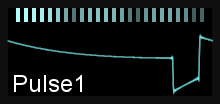
\includegraphics[scale=0.3]{5.png}
\vspace{-3em}\caption{Editing Mutable Parameters}\label{mutationparameters}
\end{wrapfigure}

You can restrict the Mutation and Recombination portions of exploration (used in Randomize, Nudge, Merge, Blend, Hill-Climb/Constrict, and Morph) to only affect a subset of parameters.  To do this, choose {\bf Edit Mutable Parameters} in the {\bf Edit} menu.  This will turn on {\it Mutable Parameters} mode (you'll see it in the window's title bar).  You'll note that various widgets have now been surrounded with red frames.  These widgets control synth parameters which are presently are being updated when you mutate a patch. 

You can change these of course: just click on them and you can remove them from being updated (or add them back).\footnote{Note that due to an error in Java's design, you can't click directly on a Combo Box (a pop-up menu) such as the ``Wave'' combo box in Figure \ref{mutationparameters}.  But you can click on its title (the text ``Wave'').}  You can also turn on (or turn off) all of the parameters in a category by double-clicking on the category title while in Mutable Parameters mode (the categories in Figure \ref{mutationparameters} are {\it Yamaha TX81Z}, {\it Global}, {\it LFO}, and {\it Controllers}).  Finally, you can turn on all the parameters in the entire patch editor by selecting {\bf Make All Parameters Mutable} in the {\bf Edit} menu, or conversely turn them all of by selecting {\bf Make All Parameters Immutable}.  You can also just {\bf Make Non-Metric Parameters Immutable}.

A very few parameters, such as the patch name, can't be mutated no matter what: these have been fixed to be immutable by the patch editor.  They will never have a red frame no matter how much you click them.

%The parameters you have selected will be the only ones changed when you mutate (randomize) a patch.  
%But if you turn on {\bf Use Parameters for Nudge/Merge} in the {\bf Edit} menu, then recombination (nudging, merging) will be restricted to these parameters as well.

Once you're done choosing parameters to mutate or recombine, just select {\bf Stop Editing Mutable Parameters} in the {\bf Edit} menu.  You can save your mutable parameter choices to a file: select {\bf Save Mutable Parameters...} in the {\bf Edit} menu.  You can also reload previously-saved choices with {\bf Load Mutable Parameters...}.

If you make a new patch editor with one of the {\bf New...} menu options, it will not have the same mutable parameter choices as your current editor: rather the parameters will all be reset to mutable.\footnote{It used to be that mutable parameter choices were stored in preferences and thus were persistent even if you quit and restarted Edisyn.  Unfortunately saving many things into preferences can be {\it extremely slow} in Java, particularly on the Mac.  It just isn't feasible any more.  Instead you can load and save choices, which I realize is inconvenient, though it does let you store many different options.} However if you instead select {\bf Duplicate Synth}, the current parameter choices will be copied.

\subsection{Morphing}
\label{morph}

\begin{wrapfigure}{r}{3.6in}
\vspace{-2em}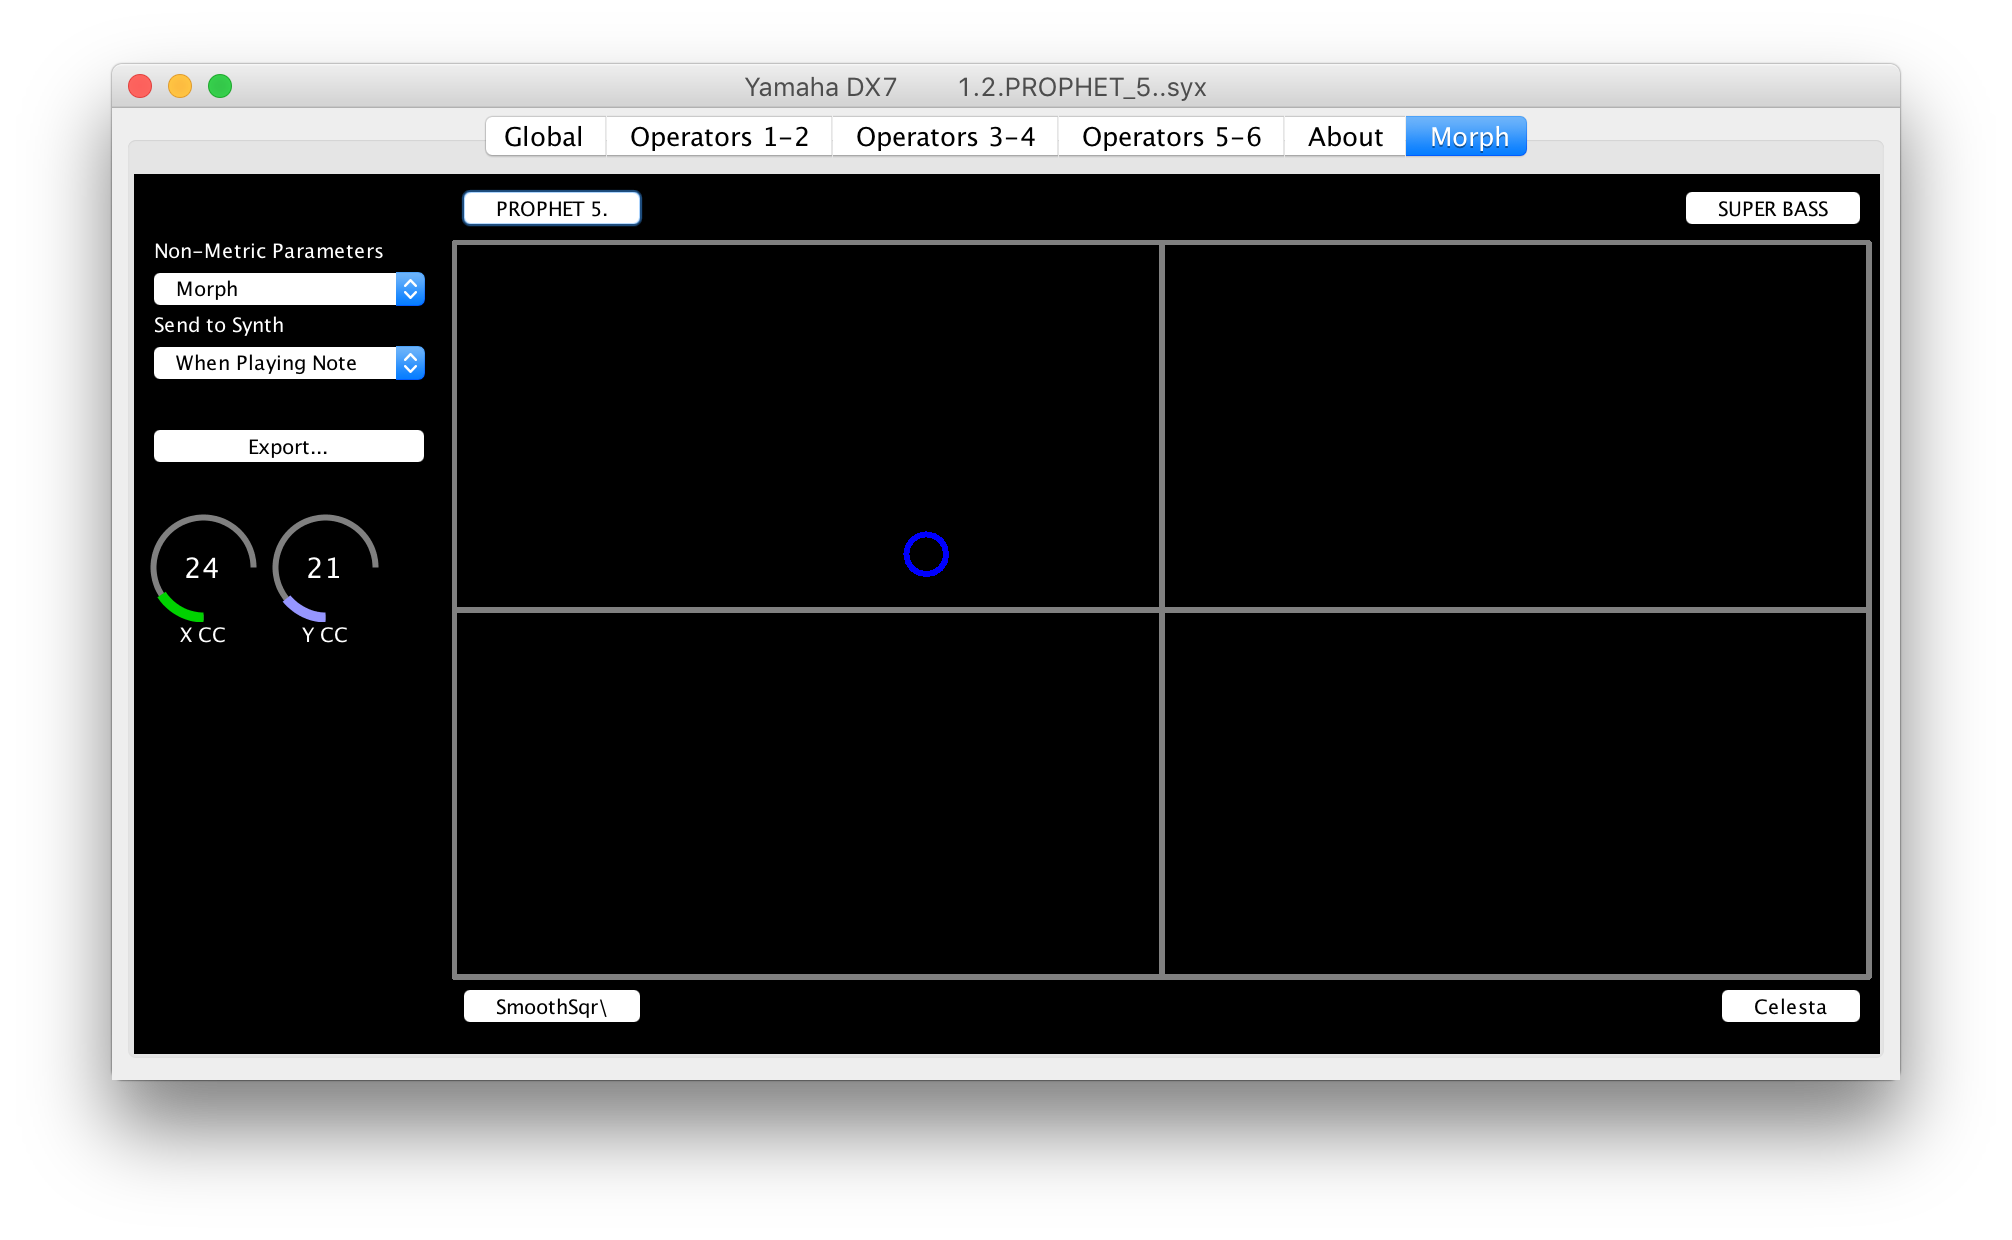
\includegraphics[scale=0.27]{Morph.png}
\vspace{-3em}
\caption{The Morpher.}
\vspace{-1em}
\label{morphpanel}
\end{wrapfigure}

The {\it Morpher} allows you to try out patches, in real time, that are a combination of four different patches. Shown in Figure~\ref{morphpanel}, the Morpher largely consists of a big rectangle with a different patch at each corner.  Once you have set up these patches, drag a joystick cursor (the blue circle) within this rectangle, and it will change the synthesizer's patch to reflect a combination of the four patches.  The closer the cursor is to a patch the more it will resemble it.

Patches are updated on your synthesizer in real time as you change the joystick cursor position.  To do this, Edisyn normally sends the entire patch to the synthesizer on the fly in the same way that ``Send to Current Patch'' is done.  Keep in mind that some synthesizers can take a bit of time to update themselves to a new patch, so depending on the synthesizer this can be either smooth or a bit jumpy.  There are other options as well.

\paragraph{Initialization} When you fire up the Morpher, it will place a copy of the current patch in the top-left corner.  You can load patches in additional corners (or overwrite the top-left corner) by clicking on their buttons and choosing one of several options:

\begin{itemize}
\item {\it Set to Editor Patch}\quad Loads the current patch in the patch editor.
\item {\it Request Current Patch}\quad Performs a {\it Request Current Patch} and, if the synthesizer responds, loads that.  This will also modify the current patch in the patch editor (you can undo it later).  If your synth is not capable of receiving current patch requests, Edisyn will tell you.\footnote{Yes, this is bad design: it ought to just disable out this option, but for irritating technical reasons this is not easy.}  Before requesting the current patch, you will probably want to temporarily turn off playing test notes because the Morpher may upload and change the patch each time it plays a new note, preventing you from changing the patch manually on your synth and then requesting it.  You can then turn modify test notes back on again to get the Morpher running.
\item {\it Request Patch...}\quad Performs a {\it Request Patch...} and, if the synthesizer responds, loads that.  This will also modify the current patch in the patch editor (you can undo it later).If your synth is not capable of receiving current patch requests, Edisyn will tell you.\addtocounter{footnote}{-1}\footnotemark\ Before requesting a patch, you will probably want to temporarily turn off playing test notes because the Morpher may upload and change the patch each time it plays a new note, preventing you from changing the patch manually on your synth and then requesting it.  You can then turn modify test notes back on again to get the Morpher running.
\item {\it Load from File ...}\quad Loads a patch from a file.
\item {\it Set to Joystick Position}\quad Loads the corner with the current joystick morphed patch.
\item {\it Clear}\quad Removes any patch from the corner.
\item {\it Swap with...}\quad Swaps the corner with another corner.
\item {\it Take from Nudge...}\quad Takes the patch from a current nudge target (1 through 4)
\item {\it Take from Hill-Climb Archive...}\quad Takes the patch from a current hill-climber archive slot (q through v).
\end{itemize}

If your synth does not support patch requests, you can go back to the current patch editor, manually request the current patch, then go back to the Morpher and initialize a corner with {\it Set to Editor Patch}.

If you don't initialize a corner, it is set to ``[Empty]''.  Empty corners do not participate in morphing.

\paragraph{Morphing} Once your corners are set up, drag the joystick cursor and listen to the result.  Here's how morphing is done.  Edisyn first computes the {\it distance} from each corner to the Joystick cursor: it's not what you think.  Think of the grid as a perfect square.  The distance is the maximum of the X distance and the Y distance from the Joystick to the corner.  The patch's metric (numerical) parameters, such as, say, Filter Cutoff, are based on the average of the four corners, each weighted by its distance.  The further the distance, the less impact the patch in that corner has on that parameter.

Non-metric parameters, such as (say) choice of filter or the PCM sampled sound played, are a different matter.  The value for a non-metric parameter is based on a strategy of your choice.  You can force the sound to draw its non-metric parameters entirely from  the current patch, from any of the four corners, or from the closest corner.  Or you can {\it Morph} the non-metric parameter.  This means that as you approach a corner, the {\it probability} that the metric parameter will be set to match the patch in that corner increases.  

\paragraph{Auditioning} As you are morphing, you'll want to hear the sound in real time: that's the whole point.  The Morpher turns repeatedly sends test notes just as the Hill-Climber does.   But the big issue is when and how often the morphed patch is sent to the synthesizer.  You have several options here, under the {\it Send to Synth} chooser:

\begin{itemize}
\item {\it When Playing Test Notes}\quad This is the default, and usually the best option.  Here, the Morpher will send the entire patch immediately before it plays a test note.  (If you have turned off sending test notes, the Morpher will never send the patch).  
\item {\it When Changing}\quad The Morpher will send the entire patch every time the joystick cursor changes.  This can be slow if the synthesizer takes a long time to update itself, but it is often the best choice if you are playing notes yourself.  Your synthesizer is unlikely to change its sound to reflect this change until the next note is played.
%\item {\it Trickle}\quad The Morpher will constantly send a single random parameter\footnote{Edisyn shuffles the parameters, then sends them in turn, then shuffles again, and so on.} to the synth.  If your synth updates itself in real-time in response to changes to these parameters, this will {\it slowly} update the patch sound of a long-playing note.  However many synths only update themselves when the next note is sounded, in which case it makes more sense to choose {\it When Playing Note}.  Note that sending individual parameters like this may take a while to fully update the patch on the synth.  Also note that this floods MIDI with messages.  You can set the {\it Trickle Rate}, which changes the number of parameters sent to the synth each trickle timestep.  By default this is 1.
%\item {\it Deluge}\quad The Morpher will constantly send the entire patch to the synth.  If your synth updates itself in real-time in response to changes to these parameters, this will {\it rapidly} update the patch sound of a long-playing note.  However many synths only update themselves when the next note is sounded, in which case it makes more sense to choose {\it When Playing Note}.  Note that this floods MIDI with messages, causing much more congestion than {\it Trickle} (there's a reason it's called {\it Deluge}).
\end{itemize}

You can turn off automatic test notes by turning off {\bf Send Test Notes} or by choosing {\bf Send All Sounds Off} in the {\bf MIDI} menu.  And you can stop Edisyn from always starting automatic play when you enter the Morpher by deselecting {\bf Morph/Hill-Climb Send Test Notes} in the {\bf Options} menu).

\paragraph{Editing} During the morphing process you might wish to modify a corner.  In addition to reloading it from various sources as discussed earlier during {\it Initialization}, you have some more options available when clicking on its button.  For example, you can swap corners with one another, which is useful for rearranging corners as you like.  You can also {\it Set to Joystick Position}, which sets the corner to the the current auditioned patch at the Joystick position, and {\it Clear}, which clears a corner of its patch (setting it to ``[Empty]'').

\paragraph{Moving the Joystick via CC}  You can set the Joystick's X and Y values via CC MIDI commands.  Simply set the X CC and Y CC dials to the CC parameter numbers to control the X and Y directions respectively.  Edisyn will remember these parameter settings in the future.

\paragraph{Autopilot}  The morpher can be set to move the cursor randomly on its own to wander about in the space.   There are three parameters which affect this.  First, when the morpher is about to move the cursor, the {\it Autopilot Jump} specifies how far the cursor will be moved.  Second, the {\it Autopilot Smooth} specifies how much the movement will be totally random (jittery) rather than a mixture of moving forward and moving randomly.  Third, the {\it Autopilot Rate} specifies how often the cursor is moved (higher is faster).  Note that if your synthesizer requires significant pauses after sending a parameter or sending a whole patch, this will significantly slow down the autopilot. 
%For example, if you are trickling, and the trickle rate is set to 20, then 20 trickles will be sent for each autopilot update, and if a single trickle is slow, the autopilot update rate will be very slow. 

\paragraph{Exporting a Patch} When you are satisfied with the current sound at your Joystick cursor, you can save it by pressing the {\it Export...} button.  Your three options are to {\it Keep Patch}, which loads the cursor patch into the current editor, {\it Edit Patch}, which loads it into a new patch editor, and {\it Save to File}, which, well, saves it to a file.

\paragraph{Quitting} Quitting the Morpher works much like quitting the Hill-Climber: choose {\bf  Stop Morphing} in the {\bf Edit} menu.

\paragraph{\color{red}Hint} Often different patches vary in pitch: for example one patch may be pitched down an octave from another.  If yo morph between these two patches, the pitch will get interpolated between them well, and it's likely you don't want a G\# when you're playing a C.  To fix this, you should turn {\it off} the parameters related to pitch: see Section~\ref{restriction} (Restricting Exploration to Only Certain Parameters) to understand how to do that.




\begin{wrapfigure}{r}{3.6in}
\vspace{-2em}\includegraphics[scale=0.27]{HillClimbPanel.png}
\vspace{-3em}
\caption{The Hill-Climber Panel}
\vspace{-2em}
\label{hcpanel}
\end{wrapfigure}

\subsection{Hill-Climbing}
\label{hillclimb}

Edisyn's {\it Hill-Climber} is another of its patch-exploration tools.  You select it by choosing {\bf Hill-Climb} in the {\bf Edit} menu.  This will add a new tab to your patch editor labelled {\bf Hill-Climb}.   When you fire up the Hill-Climber, it appears as an additional tab after your {\bf About} tab.  Whenever you select a tab other than the hill-climber tab, the hill-climber will pause; when you go back to the hill-climber tab it will resume.  You get rid of the hill-climber by selecting {\bf Stop Hill-Climbing} in the {\bf Edit} menu. 

In the Hill-Climber tab, make sure that the ``Method'' combobox is set to {\it Hill-Climb}: for other methods, see the Constrictor Section~(\ref{constrict}).

Edisyn's Hill-Climber repeatedly offers you sixteen new versions of patches and asks you to choose your top three preferences.  After you have chosen them, the Hill-Climber will try to build a new set of sounds whose parameters are similar to your choices in various ways.  The Hill-Climber builds new sounds by recombining your top three sound choices in certain ways and adding some degree of noise (mutation) to them.   If you're lucky, Edisyn will head towards regions of the synthesizer's parameter space which make sounds you like.  {\bf Hint:  You will have more success with the hill-climber if you restrict the parameters being mutated to just those you want to explore.}  Different kinds of synthesizers will also benefit from different amounts of exploration (mutation and recombination) rates.  You'll need to tweak those as necessary.

\paragraph{Candidates} This region holds the current candidate patches. When you start up the Hill-Climber, it will begin playing each candidate patch in turn.  If you don't want Edisyn to play automatically, you can turn it off by choosing {\bf Send Test Notes...} in the {\bf MIDI} menu.  (And you can prevent Edisyn from always starting automatic play when you enter the Hill-Climber by deselecting {\bf Morph/Hill-Climb Send Test Notes} in the {\bf Options} menu).  Either way, you can manually play a patch by pressing its {\bf Play} button, or by typing the key located on that button.   You can also choose which three patches you like best (in order).

\paragraph{Iterations} After you have selected your preferred patches, you can build a new set of patches from them by pressing the {\bf Climb} button.  This will also increment the iteration number.  If you don't like the patches that were built, you can try again by pressing the {\bf Retry} button.  If you'd like to back up to a previous iteration, press {\bf Back Up}.  Finally, to reset back to the very first iteration, press {\bf Reset} and choose ``From Original Patch'.

The amount of mutation noise used when generating new patches is specified by the {\bf Mutation Rate} dial.  Typically you'd select something around 5--10.  Additionally, by default the Hill-Climber lets you select from 16 candidates.  But if you press {\bf Big}, this set will expand to 32 candidates.

\paragraph{Archive} If you like a patch and you'd like to hold onto it even after hill-climbing to the next iteration, you can place it in the {\it archive}.  The archive consists of six patch locations: to copy a patch to a given archive location, click on its {\bf Options} button and select one of {\bf Archive to q} through {\bf Archive to v} (the Archive patches are so named because presently played by pressing keys q through v).  Archived patches can also be selected to participate in hill-climbing: just pick a number under a given patch.

\paragraph{Current and None} The {\it Current} category holds the patch currently being edited in your editor, and it too can be selected to participate in hill-climbing at any time.  Finally, if you select a number in the {\it None} category (number 2, say) then no patch is selected for number 2 at this time.

\paragraph{Additional Options} The {\bf Options} button holds some additional features besides just copying to the archive.  

\enlargethispage{0.5em}

\begin{itemize}
\item {\bf Keep Patch}\quad Loads the patch into the current patch in your patch editor.
\item {\bf Edit Patch}\quad Creates a new patch editor and loads the patch into that.  Note that if you edit the patch in its editor, the {\it changes you make will be automatically reflected here}.
\item {\bf Save to File}\quad Saves the patch to a file.
\item {\bf Load from File}\quad Changes the patch to one loaded from a file. 
\item {\bf Nudge Candidates to Me}\quad Nudges all the candidates towards the given patch. 
\end{itemize}

\paragraph{More Keystroke Options}

All the patches can be played by pressing their associated letter.  But additionally you can (at present) {\bf Climb} by pressing the Space Bar, {\bf Retry} by pressing the Return/Enter key, and {\bf Back Up} by pressing Backspace.

\paragraph{\color{red}Hint} Some parameters dominate how a patch sounds, and not in a good way.  On the Yamaha DX7, mutating the Pitch Envelope, per-operator Fixed Frequency, and per-operator Detune will have bad effects on a sound.  On the Oberheim Matrix 6/6R/1000, it makes no sense to allow mutation to change the overall VCA1 Volume of the sound.   Pruning certain parameters so that they cannot be mutated by the Hill-Climber will reduce the amount of junk you have to listen to, and greatly improve your hill-climbing experience. See Section~\ref{restriction} (Restricting Exploration to Only Certain Parameters) to understand how to do this.

\subsection{Constricting}
\label{constrict}

The {\it Constrictor} is similar to the Hill-Climber in many ways, yet its dynamics and behavior are quite different.   You choose the Constrictor in the same way as the Hill-Climber: by choosing {\bf Hill-Climb} in the {\bf Edit} menu.  But then in the Hill-Climb tab, change the ``Method'' combobox to {\it Constrictor}.    

The Constrictor auditions patches to you in exactly the same way was the Hill-Climber.  But you're not given the option of choosing your top three choices.  Instead, you're asked to choose which patches you {\it don't like}.  This is done by deselecting their checkboxes.  Afterwards, you click on the {\bf Constrict} button and those patches will be replaced with recombined and mutated versions of the remaining patches.  The newly recombined replacements will be moved to the front of the Candidates so you hear them first.

\begin{wrapfigure}{r}{3.6in}
\vspace{-1em}\includegraphics[scale=0.27]{ConstrictorPanel.png}
\vspace{-3em}
\caption{The Hill-Climber Panel converted for Constricting.}
\vspace{-2em}
\label{constrictorpanel}
\end{wrapfigure}

The idea behind the Constrictor is to start with a set of varied but high-quality patches\,---\,derived from well-vetted factory patches for example.  Think of these patches as the outer boundaries of a large region of the space.  As you delete patch sounds you don't like, this region slowly begins to collapse, until ultimately it converges to a single patch.

The {\it Mutation Rate} dial controls the degree of mutation rate for the constrictor.  Note that this rate is {\it different from}, and stored apart from, the hill-climbing mutation rate.  By default there is no mutation. 

\paragraph{Initialization}  For the constrictor to work, you have to initialize the Candidates with a set of varied patches.  You could load these patches one by one by clicking on each Candidates' Options button and choosing {\it Load from File}.  But there's an easier way.  Load just the first four Candidates this way, via Load from File, and then clicking on the {\bf Reset} button and choose {\bf From First Four Candidates}.  The remaining candidates (5...16, or even 5...32) will be generated from recombinations of the first four.  If you're doing 32 candidates (that is, you pressed the {\it Big} button), you might consider loading the first six candidates and then choosing {\bf From First Six Candidates}, which gives a better mix.

%\paragraph{Smooth Versus Unsmooth}
%The smooth constrictor recombines candidates by interpolating between their metric parameters.  The unsmooth constrictor recombines them by simply picking one parameter or the other from the parents.  The unsmooth constrictor makes a more noisy set of patches.  Tests have found that people like the smooth constrictor better, so I might get rid of Unsmooth in the future.

\paragraph{Using the Constrictor Along with the Hill-Climber} It's not a bad idea to start with a constrictor, constrict down to a single patch or so, and then switch over to the hill-climber and hill-climb from there.  It is a {\bf bad} idea to go from the hill-climber to the constrictor because the hill-climber restricts the candidates to a small space and the constrictor will constrict that small space almost immediately.


\ignore{
\subsection{How the Hill-Climber Makes New Sounds}

The Hill-Climber builds new sounds by recombining your top three sound choices and adding some degree of noise (mutation) to them.  Let's say that your top three sounds were sounds {\bf A, B,} and {\bf C}, and that your {\it previous} ``A'' from last time is called {\bf Z}.      You can also select only two top choices (A and B), or  single choice (A).   Figure \ref{hcfigure} explains the mechanism by which the 16 new patches are generated through various recombination and mutation mechanisms for the first 16 patches.  If you have chosen to use 32 candidate patches, then the second 16 are done exactly like the first 16, except with twice the mutation rate.

The hill-climber tries to balance coming up with mixtures of your selections as well as things well outside the searched space (balancing so-called {\it exploration} and {\it exploitation}). It also attempts to move further in the direction you had just moved, in the hopes that you'll like even more of what you had selected.


%    \begin{figure}[t]
%    \begin{center}
%    \small
%    \begin{tabular}{@{}ll@{}}
%    \multicolumn{2}{c}{\bf A, B, and C}\\
%    \hline
%    \bf Operation&\bf Mutation\\
%    A $+$ B& 1x\\
%    A $+$ C& 1x\\
%    B $+$ C& 1x\\
%    A $+$ (B $+$ C)& 1x\\
%    A $-$ B& 1x\\
%    B $-$ A& 1x\\
%    A $-$ C& 1x\\
%    C $-$ A& 1x\\
%    B $-$ C& 1x\\
%    C $-$ B& 1x\\
%    A $-$ Z& 1x\\
%    B $-$ Z& 1x\\
%    C $-$ Z& 1x\\
%    A& 3x\\
%    B& 3x\\
%    C& 3x\\
%    \end{tabular}\hspace{\fill}
%    \begin{tabular}{@{}ll@{}}
%    \multicolumn{2}{c}{\bf A, and B}\\
%    \hline
%    \bf Operation&\bf Mutation\\
%    A $+$ B& 1x\\
%    A $+$ B& 2x\\
%    A $+$ B& 3x\\
%    A $-$ B& 1x\\
%    A $-$ B& 2x\\
%    B $-$ A& 1x\\
%    B $-$ A& 2x\\
%    A $-$ Z& 1x\\
%    A $-$ Z& 2x\\
%    B $-$ Z& 1x\\
%    B $-$ Z& 2x\\
%    (A $-$ Z) $+$ (B $-$ Z)& 1x\\
%    A& 1x\\
%    A& 2x\\
%    B& 1x\\
%    B& 2x\\
%    \end{tabular}\hspace{\fill}
%    \begin{tabular}{@{}ll@{}}
%    \multicolumn{2}{c}{\bf A Only}\\
%    \hline
%    \bf Operation&\bf Mutation\\
%    A& 2x\\
%    A& 2x\\ 
%    A& 2x\\ 
%    A& 2x\\
%    A& 2x\\
%    A& 2x\\
%    A& 3x\\
%    A& 3x\\
%    A& 3x\\
%    A& 4x\\
%    A& 4x\\
%    A& 5x\\
%    A& 5x\\
%    A $-$ Z& 1x\\
%    A $-$ Z& 2x\\
%    (A $-$ Z) $-$ Z& 2x\\
%    \end{tabular}
%    \end{center}
%    \caption{Operations producing the sixteen new children each hill-climbing step.  The operations performed depend on whether the user has made  one, two, or three selections.    Each operation is followed by a certain degree of mutation.  A, B, and C are the (up to) three selections, A being most preferred and C being least.  Z is the most preferred selection the {\it previous} iteration.  The operation \(X + Y\) means to recombine X with Y, with somewhat of a bias towards X.  The operation \(X - Y\) means to find a point on the opposite side of X from Y.  The values 2x, 3x etc. aren't {\it stronger} mutation; but rather they are {\it repeated mutation operations}.  That is, 3x means to mutate, then mutate again, then mutate again.  See Figure \ref{hcfigure}.}
%    \label{hctable}
%    \end{figure}
   

\begin{figure}[t]
\begin{center}
\includegraphics[width=5in]{HillClimbingBig.pdf}
\end{center}
\caption{Recombination and Opposite-Recombination in the Hill-Climber. Shown are (left to right) basic operations performed when the user has made three (A, B, C), two (A, B), or only one (A) selections.  Z is the top selection the previous iteration (the previous iteration's A). Operations are combinations of basic Edisyn recombination procedures.  Specifically, \(A + B\) means ordinary recombination between \(A\) and \(B\), weighted towards \(A\).  Whereas \(A - B\) means opposite-recombination, finding a point on the other side of \(A\) from the location of \(B\).   Each operation is accompanied by numbers in brackets, such as [2, 3].  In this example, this means that two children will be produced using this particular operation: one (2) will be then mutated twice, and the other (3) three times.  Recombination and Opposite-Recombination are always done with a weight of 0.75; but mutation is done with a weight specified by the user on the panel.}
\label{hcfigure}
\end{figure}

When you fire up the Hill-Climber the first time, it doesn't have three candidates yet, nor does it have a Z.  So instead what it does is take your current patch and build sixteen sounds as follows:

\begin{itemize}
\item{1--4}: Four mutated versions of the current patch
\item{5--8}: Four twice-mutated versions of the current patch
\item{9--12}: Four thrice-mutated versions of the current patch
\item{13--16}: Four 4x mutated versions of the current patch
\end{itemize}

Again, if you have chosen to do 32 patches rather than 16, then the second 16 are done in the same way, but with twice the mutation rate.

\subsection{How Recombination and Mutation Work}

Edisyn's patch merging, patch mutation (randomization), nudging, and hill-climber all rely on certain low-level patch manipulation operations to do their magic.    These operations are {\bf mutation}, {\bf recombination}, and {\bf opposite-recombination}.  

All three of these operations take a {\bf weight} (a value between 0.0 and 1.0) which specifies how strong an effect the operation will have.  Sometimes this weight specified the {\it probability} that a patch parameter will change.  Other times the weight influences the {\it amount} the patch parameter will change by.

Patches are lists of parameters.   Each parameter takes one of several forms:

\begin{itemize}
\item A {\it metric parameter} can take on a value from number range, such as from 0...127.
\item A {\it non-metric} parameter can take on a value from a set of unordered elements: for example, a set of waves, or a set of filter types.
\item A {\it boolean} parameter can take on only two values (0/1, or on/off, of triangle/saw, etc.).  Boolean parameters are assumed to be non-metric parameters.
\item A {\it semi-metric} parameter has both a metric range and a non-metric range.  For example, a MIDI Channel parameter might have the metric values 1...16 plus the non-metric options OMNI and OFF.
\item Some parameters are {\it immutable}: they will refuse to be modified.  These are typically things like patch names.  You can make other parameters immutable by turning whether they can be edited on or off (see Section \ref{restriction}).
\end{itemize}

\begin{figure}[t]
\begin{minipage}{\linewidth}
\begin{minipage}[t]{\linewidth}%
\begin{algorithm}[H]
   \caption{~MutateM(Parameter \(P\) with value \(v\); {\it weight})}
   \label{alg:example}
\begin{algorithmic}
\STATE \(l, h \leftarrow\) metric min and metric max of \(P\), respectively
\REPEAT
\STATE \(\delta \leftarrow N(0,\, 0.5 \times (\frac{1}{1 - \text{\it weight}} - 1)) \times (h - l) \mod 2\)\hspace{\fill}{\it \(N(\mu, \sigma)\): Normal{\hspace{-0.2em}}}
\UNTIL{\(l - 0.5 < v + \delta < h + 0.5\)}
	\STATE{{\bfseries return}  \(v + \delta\) rounded to the nearest integer}
 %  \STATE \(q \leftarrow \text{\it weight} \times (1 + \text{metric max of \(P\)} - \text{metric min of \(P\)})\)
 %  \STATE \(l \leftarrow \max( v- \lfloor q\rfloor, \text{ metric min of \(P\)})\)
%   \STATE \(h \leftarrow \min(v + \lceil q\rceil, \text{ metric max of \(P\)})\)
%\STATE {\bfseries return} a uniform random selection from \([l, h]\)
  \end{algorithmic}
\end{algorithm}
\end{minipage}\\
\begin{minipage}[t]{\linewidth}
\begin{algorithm}[H]
   \caption{~Mutate(Parameter \(P\) with value \(v\); {\it weight})}
   \label{alg:mutate}
\begin{algorithmic}
    \IF{\(P\) is metric}
   \STATE{\bfseries return } MutateM(\(P, v\), {\it weight})
    \ELSIF{\(P\) is semi-metric and \(v\) is a metric value}
   	\IF{probability 0.5}
   		\STATE {\bfseries return } MutateM(\(P, v\), {\it weight})
	\ELSIF{probability {\it weight}}
		\STATE {\bfseries return} a random  \(p_{\text{non-metric}} \in P\)
	\ENDIF
    \ELSIF{\(P\) is semi-metric and \(v\) is not a metric value}
		\IF{probability {\it weight}}
		   	\IF{probability 0.5}
				\STATE{\bfseries return} a random \(p_{\text{metric}} \in P\)
		    	\ELSE
	    			\STATE {\bfseries return} a random  \(p_{\text{non-metric}} \in P\)
    			\ENDIF
		\ENDIF
    \ELSIF{probability {\it weight}}
			\STATE {\bfseries return} random \(p_{\text{metric}}\!\in P\)
    \ENDIF
    \STATE {\bfseries return} \(v\)
  \end{algorithmic}
\end{algorithm}
\end{minipage}
\end{minipage}
\caption{The {\bf Mutate} function, which calls the {\bf MetricMutate} sub-function as necessary for metric parameters or semi-metric parameters in the metric range.  The ``metric min'' and ``metric max'' are the maximum and minimum values in the metric range of parameter \(P\). }
\label{mutate}
\end{figure}

\paragraph{Mutation}
When a patch {\bf A} is {\it mutated}, each of its parameters is modified with some degree of random noise, or with some probability.  Figure~\ref{mutate} shows the procedure for mutating a single parameter \(P\) in a patch.  The parameter has the current value \(v\) and the user-specified {\it weight}.  The new parameter value is returned.  Mutation is used in patch randomization in nudging, and in Hill-Climbing.

Notice that if \(v\) is a metric value, and the algorithm has decided it will stay a metric value, then it uses a special sub-procedure, {\it MetricMutate}, to mutate the value to something relatively near to the original; the distance is determined by the weight.  Otherwise generally new (metric, non-metric) values are chosen completely at random with a certain probability based on the weight.


\begin{figure}[t]
\begin{minipage}{\linewidth}
\begin{minipage}[t]{\linewidth}%
\begin{algorithm}[H]
   \caption{~Recombine(Param \(P\) with values \(v, w\); {\it weight})}
   \label{alg:recombine}
\begin{algorithmic}
    \IF{both \(v\) and \(w\) are metric values in \(P\)}
    	\STATE \(q \leftarrow v - \text{\it weight} \times (v - w),\)\quad rounded towards \(w\)
    	\STATE {\bfseries return} a random uniform selection from \([v, q ]\)
    \ELSIF{probability {\it weight}}
\STATE  {\bfseries return} \(w\)
     \ENDIF
	\STATE {\bfseries return} \(v\)

%    	\IF{probability {\it weight}}
%    	    	\IF{\(v\) and \(w\) are both metric values in \(P\)}
%    			\STATE  {\bfseries return } a uniform random selection from \([v, w]\) 
%    		\ELSIF{probability 0.5}
%    				\vspace{-1.2em}\STATE\hspace{9.5em}~~{\bfseries return \(w\)}
%    		\ENDIF
%    	\ENDIF
%        \STATE {\bfseries return} \(v\)
  \end{algorithmic}
\end{algorithm}
\end{minipage}\\
\begin{minipage}[t]{\linewidth}
\begin{algorithm}[H]
   \caption{~Opposite(Param \(P\) with values \(v, w\); {\it weight})}
   \label{alg:opposite}
\begin{algorithmic}
    \IF{both \(v\) and \(w\) are metric values in \(P\)}
    	\STATE \(q \leftarrow v + \text{\it weight} \times (v - w),\)\quad rounded away from \(w\)
    	\STATE \(q \leftarrow \text{min}(\text{max}(q, \text{ metric min of \(P\)}), \text{ metric max of \(P\)})\)
    	\STATE {\bfseries return} a random uniform selection from \([v, q]\) 
 \ENDIF
        \STATE {\bfseries return} \(v\)
  \end{algorithmic}
\end{algorithm}
\end{minipage}
\end{minipage}
\caption{The {\bf Recombine} and {\bf Opposite} functions.  Each take a parameter with {\it two} values \(v\) and \(w\) (one from each patch being recombined), plus a user-specified {\it weight}.  Additionally the Opposite function takes a boolean argument, {\it flee}, which indicates whether Opposite is being presently used to flee away from \(w\).   The ``metric min'' and ``metric max'' are the maximum and minimum values in the metric range of parameter \(P\).}
\label{recombine}
\end{figure}

% this little dance is because \paragraph won't work right here and I'm not sure why
\vspace{1em}\noindent{\bf Recombination}\quad
This takes two values \(v\) and \(w\) for a given parameter \(P\) and returns a new value for \(v\).  If both values are metric, then a value is selected between them with a certain probability.  Else \(v\) either stays as \(v\) or changes to \(w\) with a certain probability.  See Figure \ref{recombine}.  Recombination is used in the patch-merge operation, as well as forming the ``plus'' operation in the Hill-Climbing procedure (see Figure~\ref{hcfigure} and Table~\ref{hctable}). 

% this little dance is because \paragraph won't work right here and I'm not sure why
\vspace{1em}\noindent{\bf Opposite Recombination}\quad
This is used to find a new patch \(Q\) which is on the {\it other side} of patch \(P\) from where patch \(S\) is.  There are two reasons you might want to do this.  One obvious reason is because you want to essentially move \(P\) away from \(S\) (so \(P\) becomes \(Q\)).  This is called {\it fleeing}: it's used in Edisyn for {\it nudging away} from a target patch.

The other reason is because you have recently moved from \(S\) to \(P\), and now you'd like to move \(P\) even {\it further} in that direction.  This is the ``minus'' operation  done the Hill-Climbing procedure (see Figure~\ref{hcfigure}).  You'll note from Figure \ref{recombine} that the Opposite procedure takes a {\it flee} argument to distinguish between your two reasons.   This largely influences what will happen if the two parameter values are the same.\footnote{Note that we assume that all metric parameters are integers, not real-valued}.
}

\subsection{Deep Learned Neural Hill-Climbing and Randomization}

The Yamaha DX7 editor has a special feature thanks to research done here at George Mason University by V.~Hoyle and myself.  Using approximately 30,000 unique DX7 patches found around the internet, we trained a special kind of deep-learned neural network called a {\it variational autoencoder}.  Using this network, we can improve both hill-climbing and patch randomization.

If you're editing a DX7, you can use the neural network in hill-climbing by selecting {\bf NN Hill-Climber} in the Hill-Climber's ``Method'' chooser.  Thereafter instead of creating children patches via recombination and mutation, Edisyn will produce them using the autoencoder.  Similarly, if (when editing a DX7) you select {\bf Edit \(\rightarrow\) Randomize \(\rightarrow\) Randomizes Using NN}, then randomization options will use the autoencoder rather than the standard mutator.

\paragraph{What's the point?}  As anyone who programs synthesizer patches knows, the space of synthesizer patches consists of small regions of good patches surrounded by lots of garbage, even regions of total silence.  The hill-climber tries many strategies to avoid presenting garbage to the user, but is only partly successful.   The goal of the autoencoder is to eliminate as much garbage and silence as possible, thus improving the chances that you'll get decent patch results.  We'd appreciate feedback as to how successful you think we were.
 
\paragraph{How does it work?}  A variational autoencoder is a special kind of neural network trained to take an incoming patch and then output the same exact patch.  The trick, however, is that it has to first squeeze the patch through a narrow data channel much smaller than the size of a standard patch.  And it must successfully do this for all 30,000 training patches fed to it: they all must be able to be squeezed down and then reconstituted at the other end as best as it can.

In order to compress all 30,000 patches, the neural network has to learn the relationships common to them, then just squeeze those relationships through the narrow neck.  This subspace of the patch space is called the {\it latent space} of the autoencoder.  Ideally the latent space just contains the stuff that makes the patches good patches in the first place: it has eliminated the features of the patch space common to garbage patches or silence.  In short, it must learn a {\it manifold}, that is, lower dimensional space folded up into the subregion of the higher-dimensional patch space where the good patches seem to reside.

Once we have trained the autoencoder, we can break it into two pieces: the {\it compression} portion, which squeezed the patch down to its bare essential features to get it through the narrow neck, and the {\it decompression} portion, which reconstituted it at the other end.  Now, what happens if we feed random ``compressed'' values into the decompression portion rather than an original patch?  It'll decompress it into a random patch somewhere in the vicinity of the trained patches (the good stuff)!  We could use this to make random patches with a high probability that they won't be garbage.  The hill-climber could also hill-climb in the space of compressed data rather than the original patch space, and so only wander around in the ``good'' regions (with luck).  And to seed the hill-climber with initial patches, we just feed them to the compression portion to get their compressed versions.

\paragraph{Can you do it on anything but the DX7?} Training an autoencoder requires a great many patches.  Most synths just don't have enough unique patches available online.  One obvious target in the future might be the Yamaha TX81Z: but it's only got around 5000 unique patches, which might not be enough.  We'll see.
 
\paragraph{About those 30,000 patches...} In Edisyn's \texttt{resources} directory, we have included a text file containing the DX7 parameters of each of those patches as numbers. Perhaps it might be useful to other researchers. 

\section{The Libriarian}
\label{librarian}

\begin{wrapfigure}{r}{3.3in}
\vspace{-2em}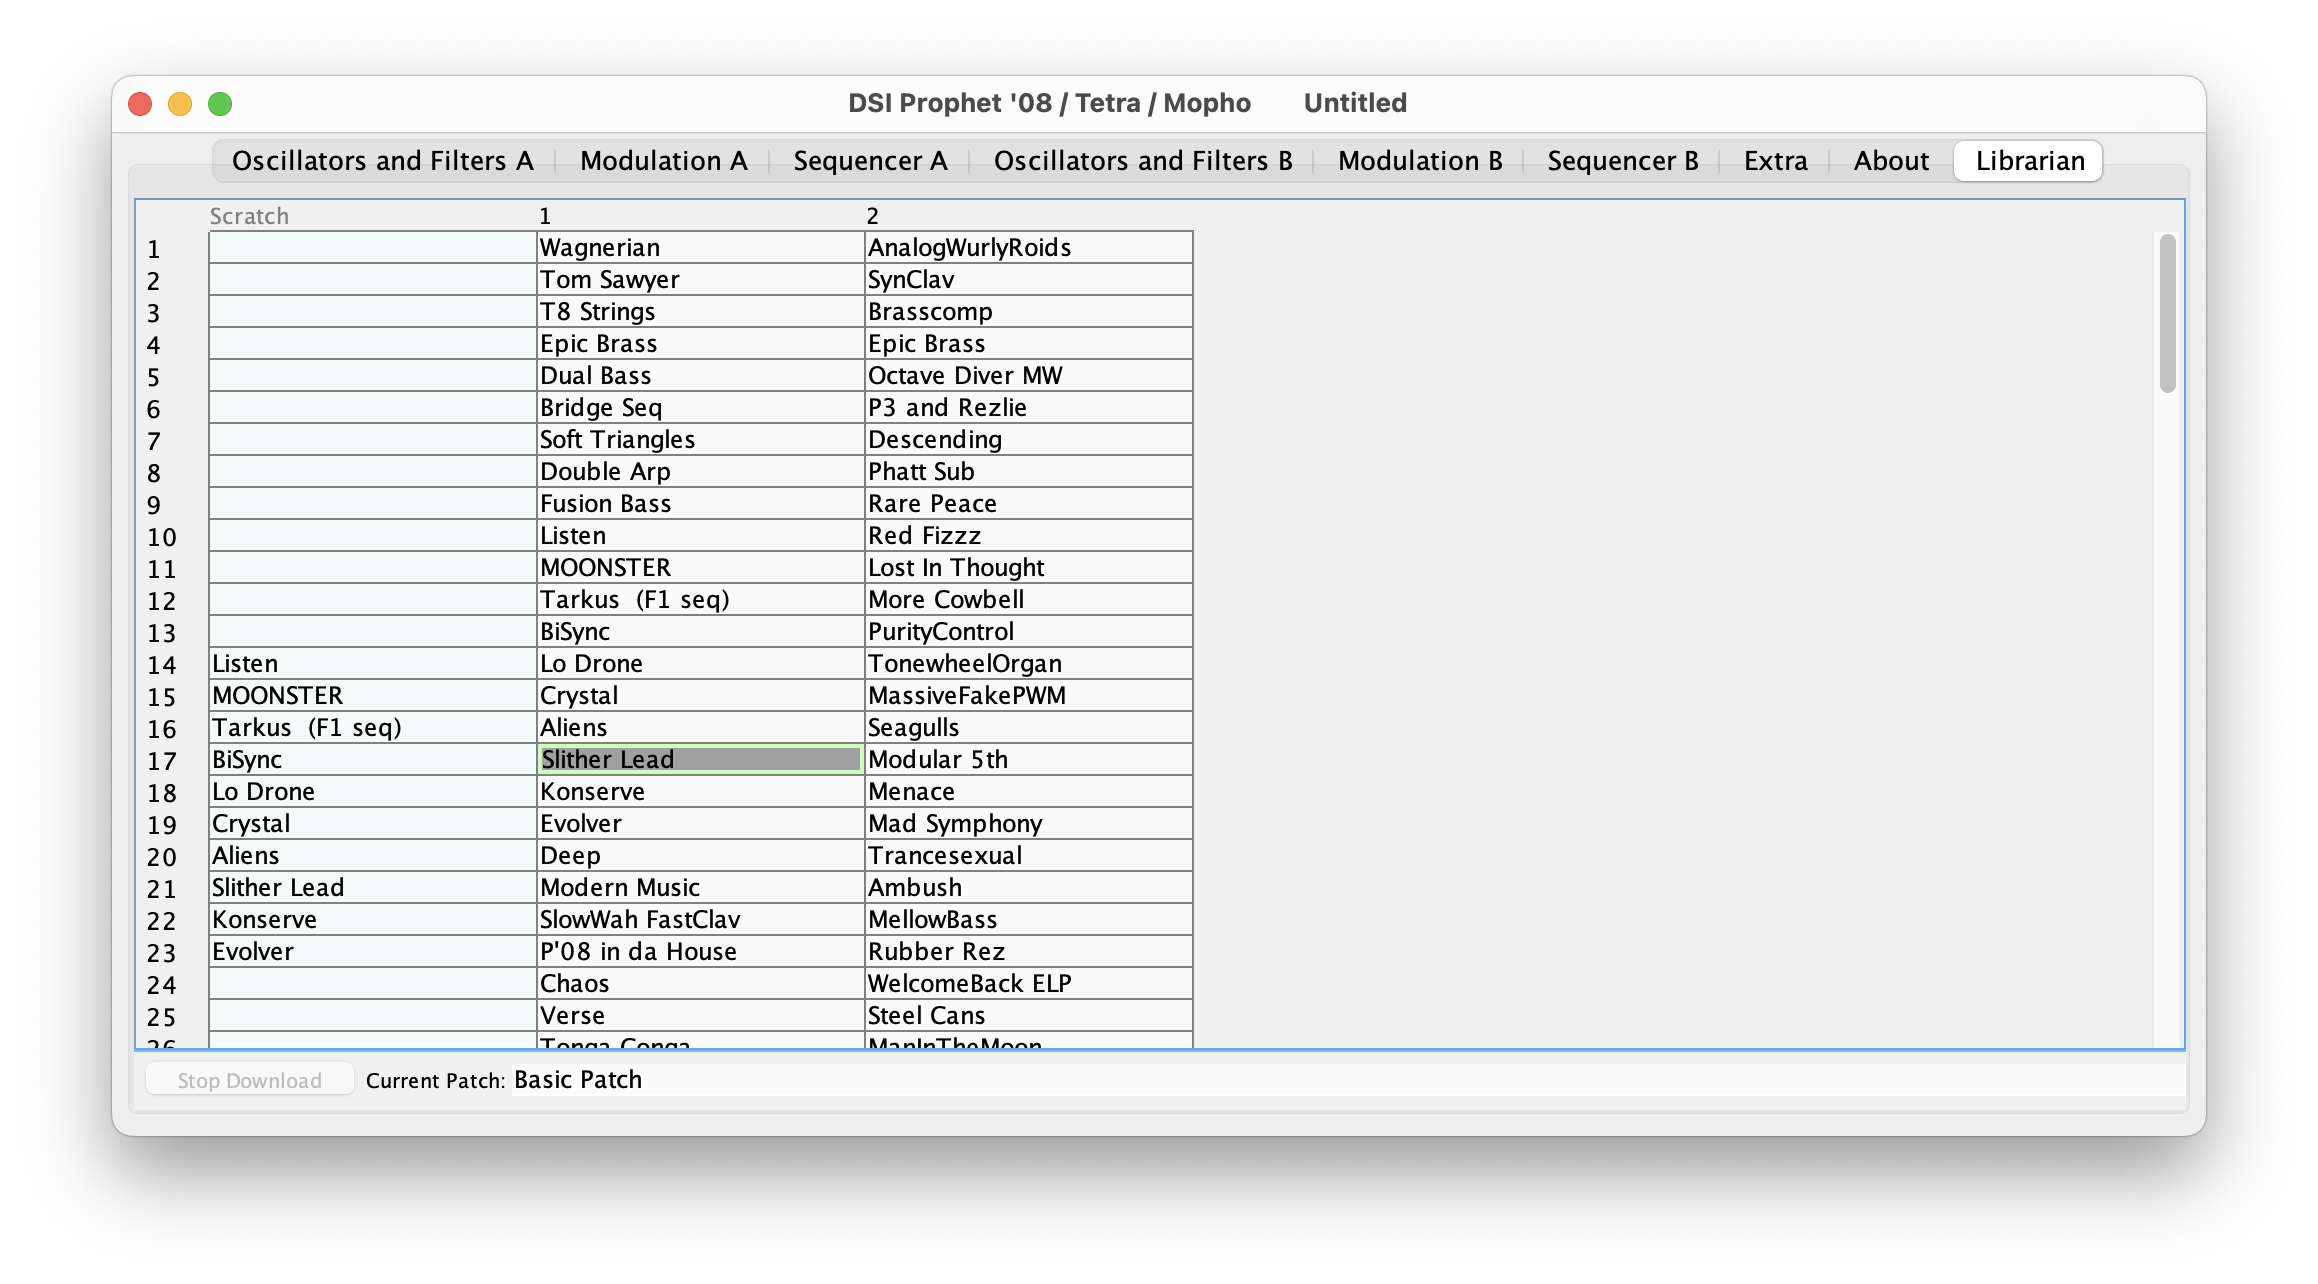
\includegraphics[width=3.4in]{Librarian.png}
\vspace{-3em}
\caption{The Librarian.}
\vspace{-1em}
\label{librarianpanel}
\end{wrapfigure}

%\hspace{0em}{\color{red}\bf Warning: The Librarian has only been tested n synthesizers, and is subject to radical change.  You may not  even have it on your version of Edisyn yet.}

Most patch editors in Edisyn sport a simple librarian.  You can call up the librarian by choosing {\bf Show Librarian} from the {\bf File} menu.  The Librarian pops up as its own tab, and looks something like what's shown in Figure~\ref{librarianpanel}, thought the particular layout will vary depending on your synthesizer. The purpose of a librarian is to allow you to load and save, rearrange, and upload or download patches in bulk.  %Edisyn's libarians are rudimentary but they should get the job done.  

The Librarian presents itself as a table with columns and rows.  Each column is a {\it bank} in your synthesizer, and each row is a {\it patch number} across all banks.  Edisyn tries to label the banks and the patch numbers like your synthesizer does.  You can rearrange and resize the bank columns.  

\paragraph{Slot Colors} 

Patch slots come in different colors depending on the situation:

\begin{itemize}
\item {\it Pale Green: the \textbf{Scratch Bank}}\quad The first column is special.  This isn't a bank in your synthesizer: it's just some extra room for you to temporarily stash stuff as you move things around via drag-and-drop.  It's not written to the synthesizer nor saved to disk.
\item {\it White}\quad Patches in locations which can be written to your synthesizer.
\item {\it Pale Magenta}\quad Patches in locations which cannot be written to your synthesizer because they're {\bf read-only} on your machine.  However you can save them to disk, and can load them from the disk or from your synth.
\item {\it Light Gray with Red Lettering}\quad Patches in locations which cannot be written to nor read from your synthesizer because they're {\bf invalid patch locations.}  Why does Edisyn provide them then?  Because some synths have banks with varying lengths or present other unusual situations which violate the rectangular table structure used by Edisyn.  You can treat them as scratch locations.
\item {\it Light Gray with Black Lettering}\quad Patches in locations which ought not be written to nor read from your synthesizer because they're {\bf ``inappropriate'' patch locations.}  You can still read/write the patches to disk while they are in these locations, but the synthesizer likely will not respond if you try to request or write them.  For example, the Proteus 2000 has four card slots which can be populated with any of 20 different read-only cards of patches.  If a card is in a slot, its ``bank'' is displayed in Pale Magenta as usual.  If a card is not in a slot, its ``bank'' is still shown, but is displayed as {\it inappropriate}: it's a real card type with legitimate patch locations, and it {\it could} be installed on a synth, so reading/writing its patches to the disk is reasonable, but accessing them on your synthesizer presently won't do anything (because it's not installed on your machine).  You can treat these spots as scratch locations if you like.
\item {\it Dark Gray}\quad Patches you have selected.
\item {\it Violet}\quad The drop location for drag-and-drop.
\end{itemize}

\paragraph{Relationship with the Editor} 

Many editor/librarian GUIs out there organize themselves so that you're presented with a librarian first, and can only edit patches once you have selected them in the librarian.  Edisyn doesn't do this: it is first and foremost an editor.  The Librarian is entirely separate from the editor and works independently of it.  For example, if you select a patch in the Librarian and arrange for it to be edited in the editor, the editor is editing a {\it copy} of the patch, not the original patch in the librarian. They're not linked.  You'll have to copy it back to the librarian once you have finished editing it.

\paragraph{Jumping to and Hiding the Librarian}
 
Some other software packages display the librarian and the editor at the same time, so you can select a patch in the librarian list and immediately see it displayed in the editor.  Edisyn doesn't do this.  However, if you double-click on a patch to see it in the editor, you can go back to the librarian very quickly by choosing {\bf Show Librarian} again (or better yet, pressing Command-L on the Mac or Control-L on Windows/Linux).

You can hide the Librarian by selecting {\bf Hide Librarian} in the {\bf Librarian} menu.  The data doesn't go away: if you reopen it, you'll be right back where you left off.


\subsection{Loading and Downloading} 

\paragraph{Loading Patches into the Librarian from a File}

If you open a bulk or bank sysex file, you'll be given the option (among other things) to load the data into your current Librarian or into one attached to a new editor.  If the Librarian isn't already open, it'll be opened for you.

\paragraph{Downloading Patches into the Librarian from your Synthesizer}

Usually you do this by selecting one of the {\bf Download...} options in the Librarian.  As the patches are loaded, they appear in the Librarian.  You can also select {\bf Batch Download} from the {\bf File} menu and select the {\bf To Librarian} option.  Alternatively, if you send Edisyn a Bank Sysex message from your synthesizer, Edisyn will give you the option to load the bank into the Librarian or into a new Librarian. 

While the patches are loading, the window will say {DOWNLOADING}.  If you need to prematurely stop downloading, just click on the {\bf Stop Download} button in the Librarian.  Alternatively you can select {\bf Stop Downloading Batch} from the {\bf File} menu.

{\color{red}\bf Individual downloading from a synthesizer is often quite slow} because many synths take a long time to switch to new patches and download them one at a time.  I'd suggest downloading your whole synthesizer once and saving it as a file, which would make things easier to edit in the future.

\paragraph{Fast Downloading}

Normally if you download a range of patches, a bank, or, all the patches, Edisyn will request each patch one by one, carefully and slowly.  However a few synthesizers are capable of rapidly dumping banks of patches, or all stored patches, in response to a special request.  If your synthesizer can do this, you may see the menu items {\bf Request Bank from Synth} or {\bf Request All Patches from Synth}.


\paragraph{Where Loaded Patches Go}

If you load a single patch from disk, it'll go to the editor.  But if a single patch arrives from the synth while the librarian is open, it'll go in the librarian rather than the editor.  %You can drag it from the {\it Current Patch} field into the librarian.

If you load a range of patches, the Librarian will try to be smart about it.  If the patches come with locations, the Librarian will put them in their locations.  If they don't, it'll stick them in order starting with your first bank.  

If you load one or more entire banks, either from disk or because your synthesizer sent Edisyn a bank sysex, Edisyn will stick them in the right place.  If the bank message indicates which bank it is, Edisyn will put them it in the right place.  Otherwise it'll put it in the first bank.



\subsection{Editing the Library} 

\paragraph{Selecting Patches and Moving Them Around}

Once you have patches loaded into your Librarian, you can select a range of patches in a given bank by dragging the mouse over them, or by using the up/down cursor keys in combination with Shift.  Alternatively you can double-click on the bank name (the column header) and all the patches in the bank will be selected.

After you have selected a patch range, you can drag it from one column to another.  Dragging will {\bf move} the patches to the new location, overriding the patches you dropped them on top of.  If you hold down the Control key while dragging (on the Mac you can also hold down the Option key), the you will instead {\bf copy} the patches: copies will move to the new location but the originals will stay put.  Finally if you hold down the Control and Shift keys while dragging, the drag cursor changes to Java's ``link'' cursor:   Edisyn uses this final mode to indicate that you will {\bf swap} the patches with the ones they're being dragged on top of.

Drag and Drop isn't restricted to just one Librarian: if you have two Librarians open for the same synthesizer, you can drag patches from one to the other. 

Java's table facility is weird about selecting and dragging table cells, but the general rule is this: you must first select a patch or patch range, then {\it let go of the mouse,} before you can go back and drag it. Additionally, when you drag a region, Java is particular about where the dragged region will get dropped.  For example, if you selected a region of ten cells, then clicked on the third cell in the region and dragged it, Java will highlight a drop cell location in pale violet.  This location will be where the third cell will go; and this in turn will determine where the rest of the region will be dropped.   If the region can't fit in that position, then the drop cell won't get highlighted.  If this is confusing to you, I suggest always dragging from the first cell in the selected region: then the drop location will be where the beginning of the region will get dropped.

\paragraph{Renaming Patches}  Select a patch and press Return.  If the patch can be renamed in place, the patch's name editor will pop up.  Note that you can't name empty slots in the Librarian.

\paragraph{Moving Patches to and from the Editor}

The Editor is completely separate from its Librarian.  Changing a patch in the editor doesn't change it in the Librarian, and loading a new patch in the Librarian doesn't overwrite it in the Editor.   The Editor's current patch is shown in the Librarian as the {\bf Current Patch}.  If you want to copy the Editor's current patch to the Librarian, just drag the Current Patch field into a slot in the Librarian.  

If you want to edit a patch from the Librarian, select a patch and choose {\bf Edit Patch in This Editor} from the {\bf Librarian} menu.  Alternatively you can just double-click on the Librarian patch.  This switches to the Editor for your convenience.  You can also drag the patch from the Librarian to the Current Patch field to load it into the Editor without switching to the Editor.  To edit a patch in a new Editor, select the patch and choose {\bf Edit Patch in New Editor} from the {\bf Librarian} menu.

\paragraph{Clearing Patches}

To clear a patch or a range of selected patches, select the range and press Backspace or Delete.  Alternatively you can choose a {\bf Clear Selected Patches} from the {\bf Librarian} menu.  

To clear a bank, select a patch in the bank and choose {\bf Clear Bank} from the {\bf Librarian} menu.  If there's only one bank, you don't even have to select the bank.

To clear a everything in the Librarian, select {\bf Clear All Patches} from the {\bf Librarian} menu.

\paragraph{Undo and Redo}

The Librarian has its own Undo and Redo stack independent of the editor.  You can undo or redo actions by clicking the Undo and Redo buttons.  Alternatively you can just choose {\bf Undo Librarian Action} or {\bf Redo Librarian Action} in the {\bf Edit} menu.

If you drag patches from one Librarian into another, you have affected {\it two different} Undo/Redo stacks.  Choosing Undo in one Librarian will undo the effect there, but the other Librarian's changes will stay as they are unless you also choose Undo in that Librarian as well.

\paragraph{Setting Bank Names}  A very small set of synthesizers (currently just the Yamaha FB-01) allow you to change the name of the bank.  You can do this by triple-clicking on the current bank name (the column header).

\paragraph{Exploration Tools} If you have selected a group of patches, you can route them to be Nudge targets, Morph targets, or the initial values of the Hill-Climber by choosing {\bf To Nudge Targets}, {\bf To Morph Targets}, or {\bf To Hill-Climber} respectively.     Sending a set of patches to the Hill-Climber is particularly useful as a start for the Constrictor variation.  The Librarian also has its own unique exploration tool, {\bf mixing}, which lets you blend a potentially large number of patches into one single patch or a bank of patches.  See the {\bf Mix} and {\bf Remix Banks} paragraphs in Section~\ref{explorationtools} for discussion of this.

\subsection{Saving to Disk and Writing to Your Synthesizer} 

\paragraph{Saving Patches to a File}

To save a patch or a range of selected patches to a single file or collection of files, select the range and choose {\bf Save Selected Patches...} from the {\bf Librarian} menu.

To save a bank of patches to a single file, select the a patch in the bank and choose {\bf Save Bank...} from the {\bf Librarian} menu.  Some synthesizers can save out banks with a single bank sysex message: Edisyn will use this if it's available. Otherwise, it'll just write each patch separately to the file.

To save all patches in the Librarian  to a single file or collection of files, choose {\bf Save All Patches...} from the {\bf Librarian} menu.  Many synthesizers can save out banks either with a single bank sysex message or as individual patch sysex messages.  Edisyn will give you the option if it can.  Note that saving out patches first involves building their sysex, and for some synthesizers this may take several seconds if you're saving {\it all} the patches.  Be patient: Edisyn isn't hung.

\paragraph{Writing Patches to your Synthesizer}

To write a patch or a range of selected patches to your synthesizer, select the patch or range and choose {\bf Write Selected Patches to Synth} from the {\bf Librarian} menu.  This writes the patches as if you had loaded each one in the editor and chosen {\bf Write to Patch...}.  

Note that some synthesizers (such as the Yamaha DX7) cannot do this: you can only write whole banks to them.  So, to write a bank of patches to your synthesizer, select the a patch in the bank and choose {\bf Write Bank} from the {\bf Librarian} menu.  This writes the whole bank of patches to the synthesizer.  On some synthesizers (like the Yamaha DX7) this will use a special bank-writing sysex message. For other synthesizers, it'll just write each patch separately.

To write all patches to your synthesizer, choose {\bf Write All Patches} from the {\bf Librarian} menu.  On some synthesizers (like the Yamaha DX7) this will employ a special bank-writing sysex message. For most synthesizers, it'll just write each patch separately.  

Keep in mind that if you choose the {\bf Write to Patch...} or {\bf Send to Current Patch} menu options from the {\bf MIDI} menu, this will write the current patch in the {\it editor}, not in the Librarian, even if you have selected a single patch.  It probably isn't what you wanted to do.

In order to receive patches from Edisyn, your synthesizer may need to be set up properly, such as turning off memory protection. See your patch editor's About Panel for instructions.

\paragraph{Exporting to Text}
Maybe you want to list your library in your blog?  Select {\bf Export Names to Text...} from the {\bf Librarian} menu, and Edisyn will dump out all the patch names, plus their patch locations, one per line, to a text file.



\newcommand\samefootnote{\addtocounter{footnote}{-1}\footnotemark}
\newcommand\backfootnote[1]{\addtocounter{footnote}{-#1}\footnotemark\addtocounter{footnote}{#1}\addtocounter{footnote}{-1}}
\newcommand\cm{\checkmark}

\begin{table}[p]
\vspace{5em}
\begin{center}
{\footnotesize
\begin{tabular}{rllllllllll}
&
\begin{sideways}Send Parameter\end{sideways}&
\begin{sideways}Receive Parameter\end{sideways}&
\begin{sideways}Request Specific Patch\end{sideways}&
\begin{sideways}Request Current Patch\end{sideways}&
\begin{sideways}Send to Current Patch\end{sideways}&
\begin{sideways}Write to Specific Patch\end{sideways}&
\begin{sideways}Change Mode\end{sideways}&
\begin{sideways}Receive Error or Ack\end{sideways}&
\begin{sideways}Standard Sysex File\end{sideways}\\[0.5em]
\hline\\[-0.5em]
%Futuresonus Parva&{\cm}&{\cm}&{\cm}&{\cm}&{\cm}&{\cm}&&&\\
Alesis D4/DM5&{\cm}*&&{\cm}&&{\cm}&{\cm}& & &{\cm}            \\
Audiothingies Micromonsta&{\cm}&{\cm}&&&&{\cm}*& & &{\cm}            \\
ASM Hydrasynth&{\cm}&{\cm}*&&&&{\cm}& & &{\cm}            \\
Casio CZ&&&{\cm}&{\cm}&{\cm}&{\cm}& & &{\cm}*            \\
DSI Prophet '08/Mopho/Tetra&{\cm}&{\cm}&{\cm}&{\cm}&{\cm}&{\cm}& & &{\cm}            \\
E-Mu Morpheus/UltraProteus&{\cm}& &{\cm}& & &{\cm}& & &{\cm}            \\
E-Mu Proteus&{\cm}& &{\cm}& & &{\cm}& & &{\cm}            \\
E-Mu Proteus 2000&{\cm}&{\cm}&{\cm}&{\cm}&{\cm}&{\cm}& &{\cm}&{\cm}            \\
E-Mu Planet Phatt/Orbit/Carnaval/Vintage Keys&{\cm}& &{\cm}& & &{\cm}& & &{\cm}            \\
JL Cooper MSB Plus/Plus Rev2& & &{\cm}&{\cm}& &{\cm}& &&{\cm}            \\
Kawai K1/K1r/K1m&{\cm}*& &{\cm}& & &{\cm}& &{\cm}&{\cm}            \\
Kawai K4/K4r&{\cm}*& &{\cm}& &{\cm}&{\cm}& &{\cm}&{\cm}            \\
Kawai K5/K5m&{\cm}&{\cm}&{\cm}& & &{\cm}& &{\cm}&{\cm}            \\
Korg Microsampler&{\cm}*&{\cm}*& & & & &  &  &         \\
Korg SG Rack&&&{\cm}&{\cm}&{\cm}&{\cm}&{\cm}& &{\cm}\\
Korg Volca Series&{\cm}*&& & & & &  &  &         \\
Korg Wavestation SR&{\cm}&&{\cm}&{\cm}*&{\cm}*&{\cm}&{\cm}*& &{\cm}\\
M-Audio Venom&{\cm}&&{\cm}*&{\cm}&{\cm}*&{\cm}*&{\cm}*&{\cm}&{\cm}*\\
Novation Drumstation/D Station&&&&&{\cm}*&{\cm}*& & &{\cm}          \\
Novation SL&&&&&{\cm}&{\cm}&&&{\cm}*	\\
Oberheim Matrix 1000&{\cm}&{\cm}&{\cm}& &{\cm}*&{\cm}& & &{\cm}          \\
PreenFM2&{\cm}&{\cm}&{\cm}&{\cm}&{\cm}& & & &\\
Red Sound DarkStar/DarkStar XP2&&&&&{\cm}&{\cm}& & & {\cm}           \\
Roland D-110&{\cm}& &{\cm}*&{\cm}*&{\cm}*&{\cm}*& & &{\cm}          \\
Roland JV-80/880&{\cm}& &{\cm}&{\cm}&{\cm}&{\cm}& & &{\cm}*          \\
Roland U-110&{\cm}& & &{\cm}&{\cm}&{\cm}& & &{\cm}*          \\
Roland U-220&{\cm}& &{\cm}&{\cm}&{\cm}&{\cm}& & &{\cm}*          \\
Sequential Prophet Rev2&{\cm}&{\cm}&{\cm}&{\cm}&{\cm}&{\cm}& & &{\cm}            \\
Waldorf Microwave II/XT/XTk&{\cm}&{\cm}&{\cm}&{\cm}*&{\cm}&{\cm}&{\cm}& &{\cm}            \\
Waldorf Blofeld&{\cm}*&{\cm}*&{\cm}&{\cm}*&{\cm}&{\cm}& & & {\cm}            \\
Waldorf Kyra&{\cm}&{\cm}&{\cm}*&{\cm}*&{\cm}*&{\cm*}& & & {\cm}*            \\
Waldorf Pulse 2&{\cm}&{\cm}&{\cm}&{\cm}&{\cm}&{\cm}& & &{\cm}\\
Waldorf Rocket&{\cm}&{\cm}& &{\cm}*&{\cm}*& & & &           \\
Yamaha DX7 Family&{\cm}&{\cm}&{\cm}*&{\cm} & & &  & &{\cm}            \\
Yamaha 4-Op Family&{\cm}*& &{\cm}&{\cm}&{\cm} & &  & &{\cm}*            \\
Yamaha FB-01&{\cm}*& &{\cm}&{\cm}&{\cm}&{\cm}*&  & {\cm}&{\cm}*            \\
Yamaha FS1R&{\cm}&{\cm}&{\cm}&{\cm}& &{\cm}& & &{\cm}            \\
Yamaha TG33/SY22/SY35&{\cm}*& &{\cm}&{\cm}&{\cm}& &  & &{\cm}            \\
\end{tabular}
}
\\[1em]
* {\it With significant caveats or restrictions}
\end{center}
\vspace{-1em}
\caption{Patch Editor Capabilities}
\label{patcheditorcapabilities}
\end{table}

\section{Building a Patch Editor}

So you want to write a patch editor?  They're not easy.  But they're fun!  Here are some hints. 

\subsection{Understand What You're Getting Into}
\label{inconsistent}

Understand that Edisyn can only go so far to help you in writing a patch editor: the synthesizer sysex world is an inconsistent, buggy mess.

For example, the Waldorf Blofeld's multimode sysex is undocumented and must be reverse engineered.  The PreenFM2 bombs when it receives out-of-range values over NRPN, but happily sends them to you.  The PreenFM2 has sysex files for its patches, but they are undocumented and are basically unusable memory dumps  of IEEE 754 floating-point arrays.  The Yamaha 4-Op family (such as the TX81Z) requires not one but up to {\it four} separate sysex patch dumps in a row, in order to be backward compatible with an earlier synth family nobody cares about: they are also incapable of writing a patch (likewise the PreenFM2).    The Kawai K4's sysex documentation is riddled with incredible numbers of errors.    The Matrix 1000 accepts patch names but doesn't store or emit them: it just ignores them.  The Red Sound DarkStar has extremely, {\it extremely} limited sysex.  The  AudioThingies Micromonsta can only read or write patches when rebooted into a special mode.  The Korg Wavestation SR incredibly sends parameters as {\it text strings} embedded in sysex.  Synths often pack multiple parameters into the same byte, making it impossible to update just a single parameter: you have to update five at a time.  There are multiple different strategies for packing data of size 8 bits and up.  Some synths, like the Futuresonus Parva, DSI Prophet '08, and Yamaha DX7, are highly regular in their format, while others, like the infamous Korg Microsampler, require custom tables for nearly every parameter.

Figure~\ref{patcheditorcapabilities} is a little table of the current patch editors for Edisyn, and various Edisyn capabilities that they can or cannot take advantage of.  I particularly love how the Korg Microsampler and the Korg SG are disjoint in their abilities; yet they're from the same company.   Long story short, you'll probably have to do a lot of customization.  I've tried to provide many customization options in Edisyn.  If you need something Edisyn doesn't provide, contact me.


\subsection{Setting Up the Development Environment}

Still not scared away? Let's start by getting Edisyn set up for development.  Probably the easiest way to fire up Edisyn for purposes of testing is as a build directory.  You just need to add two items to your CLASSPATH:

\begin{enumerate}
\item The {\tt coremidi4j-1.5.jar} file, located in the {\tt libraries/} folder (you can move it where you like).  This jar file contains the CoreMidi4J library, which enables sysex to work properly on Macs (you'll need it for non-Macs too).

\item The {\tt trunk} directory.  This parent directory holds the {\tt edisyn} package.  Or if you like, make some other directory {\tt foo} and move (or link) {\tt edisyn} into that directory, then add {\tt foo} to your CLASSPATH.
\end{enumerate}

Now you can compile Edisyn with\ \ \  {\tt javac~edisyn/*.java~edisyn/*/*.java~edisyn/*/*/*.java}\\
You can then run Edisyn as\ \ \  {\tt java edisyn.Edisyn}

\subsection{Creating Files}

Let's say you're adding a single (non-multimode) patch editor for the Yamaha DX7.  Understand that there {\it already} is such an editor, but it's a good exercise to understand the code perhaps.

Make a directory called {\tt edisyn/synth/yamahadx7}.  This directory will store your patch editor and any auxiliary files.  Next copy the file {\tt edisyn/synth/Blank.java} to {\tt edisyn/synth/yamahadx7/YamahaDX7.java}.  That'll be your patch editor code.  You need a separate ``recognizer'' Java file as well\,---\,you can copy the file {\tt edisyn/synth/BlankRec.java} to {\tt edisyn/synth/yamahadx7/YamahaDX7Rec.java}.  This file consists of the code sufficient to recognize a sysex message as belonging to the DX7 without having to instantiate an entire DX7 synth instance, which is costly.  Also copy the file {\tt edisyn/synth/Blank.html} to {\tt edisyn/synth/yamahadx7/YamahaDX7.html}.  This will be the ``About'' documentation for your file.  You'll eventually fill it out.

Modify the {\tt YamahaDX7.java} file to have the proper class name and package.  Then edit the {\tt edisyn/synth/Synths.txt} file.  Add to that file a line like this:\\
\\
{\tt edisyn.synth.yamahadx7.YamahaDX7\textit{\qquad[tab]\qquad}Yamaha DX7}\\
\\
Now Edisyn knows about your (currently nonexistent) patch editor class and also the name which should appear in the menu.  Finally, implement the {\tt getSynthName()} and {\tt getHTMLResourceFileName} methods in your class file, along these lines:

\begin{verbatim}
public static String getSynthName() { return "Yamaha DX7"; }
public static String getHTMLResourceFileName() { return "YamahaDX7.html"; }
\end{verbatim}

It doesn't matter if {\tt YamahaDX7.html} doesn't exist yet.

\subsection{Getting the UI Working}

This is mostly writing the class constructor and subsidiary functions.  Typically you will create one {\tt SynthPanel} for each tab in your editor.  A SynthPanel is little more than a JPanel with a black background: you can lay it out however you like.  However Edisyn typically lays it out as follows:

\begin{enumerate}
\item At the top level we have a {\bf VBox}.  This is a vertical Box to which you can add elements conveniently.  You can also designate an element to be the {\bf bottom} of the box, meaning it will take up all the remaining vertical space.
\item In the VBox we will place one or more {\bf Categories}.  These are the large colorful named regions in Edisyn (like ``LFO'' or ``Oscillator''). 
\item Typically inside a Category we'd put an {\bf HBox}.  This is a horizontal box to which you can add elements.  You can also designate an element to be the {\bf last item} of the box, meaning it will take up all the remaining horizontal space.  By doing this, the Category's horizontal colored line nicely stretches the whole length of the window.\footnote{There is an HBox (and VBox) option for designating the {\it first} element to take up all the space.  You still add the item using the addLast(...) method though.}
\item Inside the HBox you put your widgets.  You might lay them out with additional VBoxes and HBoxes as you see fit. It's particularly common to one or more small widgets (check boxes, choosers) in a VBox, which will cause them to be top-aligned rather than vertically centered as they would if they were stuck directly in the HBox.  It's helpful to look at existing patch editors to see how they did it.
\item If you need multiple rows, you should put a VBox in the Category, and then put HBoxes inside of that.
\item You might have multiple Categories on the same row.  To do this, just put them in an HBox.  Make sure the final Category is designated to be the Last Item of the HBox.  You'd put this HBox in the top-level VBox instead of the Categories themselves.
\end{enumerate}

The first category is the {\bf Synth Category}.  It is typically named the same as {\tt getSynthName()}, its color is {\tt edisyn.gui.Style.COLOR\_GLOBAL}, and contains the patch name and patch/bank information, and perhaps a bit more (for example, Waldorf synthesizers have the ``category'' there too).

To the right of the first category is usually (but not always) various global categories.  They're usually {\tt edisyn.gui.Style.COLOR\_A}.

If you have additional categories, you might distinguish them using {\tt edisyn.gui.Style.COLOR\_B}, and eventually {\tt edisyn.gui.Style.COLOR\_C}.

You can lay out the rest of the categories as you see fit.

\paragraph{Think about Parameters}

Synthesizer parameter values will be stored in your Synth object's {\bf Model}.  These parameters will be stored in your synth's {\bf Model} object.  Each parameter has a {\bf Key}.  Edisyn traditionally names the keys all lower case, plus numbers, with no spaces or hyphens or underscores, and tries to keep the keys fairly similar to how your synth sysex manual calls them.  They're usually described with a category descriptor (such as {\tt op3} and then the parameter name proper (such as {\it envattack}), resulting in the final key name {\it op3envattack}.  Various global parameters are just the parameter name: for example, it's standard in Edisyn that the patch name be just called {\it name}, the patch number is called {\it number}, and the bank number is called {\it bank}.

Often parameters (as set by widgets) are exactly the same as the various elements you send and receive to the synthesizer.  But sometimes they're not.  Many synthesizers pack multiple parameters (like LFO Speed \(+\) Latch) together into a single variable, which is very irritating.  You want to lay out what the {\it real} parameters of your synthesizer are, that the user would be modifying, not what you'd be packing and sending to the synth.

Another issue is how your synthesizer interprets values sent over sysex or NRPN.  Consider BPM for a moment.  Perhaps your synthesizer has BPM values of 20...300, and there are missing values (for example, there's no 21).  The actual values are mapped to the numbers 0...127.  What values should you store?  In my patch editors, I store the values in the model as 0...127, which makes it easy to emit them.  But then I have to have an elaborate conversion function to map them to 20...300 for display on-screen.

Also some synthesizers have holes in their ranges.  For example, they might permit the values 0...17 and the values 20...100, but do not permit 18 and 19.  What to do then?  You probably ought to compact them to be contiguous between some min and max: for example, you might compact it to 0...98.  When displayed, use a custom displayer, and when emitting or parsing them, you'll have to map them to your internal representation accordingly. 

In summary: your internal parameters ought to have contiguous ranges and should make sense from the user's perspective and not the synthesizer's weird parsing perspective.

So how to set parameters?  You usually don't add the key yourself, though you could.  Instead, normally you tell the widget the name of the parameter it's modifying (the key), and it adds it to the model on its own.  Parameters are either {\bf strings} or are {\bf numbers}.   Numerical parameters all have a {\bf min} and a {\t max} value, inclusive: usually the widget will set those for you.  They also may have a {\bf MetricMin} and  {\bf MetricMax} value, and you may need to set those manually.  

MetricMin and MetricMax work like this.  Some numerical parameters are {\bf metric}, meaning they're a range of numbers where the order matters, such as 0--127.  Other numerical parameters are {\bf categorical} (or ``non-metric''), meaning that the numbers just represent an ID for the parameter.  For example, a list of wavetables is categorical: it doesn't {\it really} matter that wavetable 0 is ``HighHarm3'': it's just where it's stored in your synth.  

Edisyn is smart about mutating and recombining metric parameters, but for non-metric ones it just picks a new random setting.  Sometimes your parameters are {\it both} metric and non-metric.  For example, some parameter might have the values 1--32 plus the non-metric values ``off'' (0), ``uniform'' (17), and ``multi'' (18), or whatever.  In this case, your min is 0 and your max is 18.  But your {\it metric min} is 1 and your {\it metric max} is 16.  This tells Edisyn that values outside the metric min / metric max range should be treated as non-metric.\footnote{What if your synth has metric values on the outside and non-metric value on the inside? Edisyn can't handle that.  Thankfully I've not seen it yet.}  If you have this situation, you'll need to set the Metric Min and Metric Max manually.

Parameters can be declared {\bf immutable}, meaning Edisyn can't mutate them or cross them over at all.  Also, all string parameters are automatically immutable.  You'll need to declare the others.

\paragraph{Parameter Conventions}

There are by convention three standard parameter names:

\begin{itemize}
\item {\bf number}\quad Patch number, always starting at 0
\item {\bf bank}\quad Patch bank, always starting at 0
\item {\bf name}\quad Patch name, a string
\end{itemize}

These are all optional.  If your synthesizer doesn't have (say) a notion of a bank, then that parameter should not exist at all.

Parameters in general by convention are a combination of lower-case letters and numbers.  No hyphens, no spaces, no underscores or other punctuation.  The numbers serve to distinguish between identical hierarchical objects (like multiple envelopes or multiple voices).  Conventionally Edisyn parameter names are 1-indexed so as to match with common synthesizer parameter names in sysex documentation.

Here are some examples:

\begin{itemize}
\item midichannel
\item lfo2rate
\item env3level2
\item voice4env3level2
\item voice4env3level2sign
\end{itemize}


\paragraph{Copying and Distributing Parameters}

If your synth has multiple copies of the same category (for example, multiple LFOs), you can {\bf copy} parameters wholesale from one category and {\bf paste} them onto another, or {\bf distribute} a parameter value to similar parameters within a category.  Furthermore you can {\bf copy} parameters from one tab to {\bf paste} onto another.  Finally, individual categories, tabs, and the entire patch can be {\bf reset}.    You can get all of this to work as long as your parameters follow a hierarchical convention as discussed here.

When one category is {\bf pasted to another category}, each of its parameters is compared each parameter of the other category to see if they {\bf match}, and if they do, then the values are copied to the other category's parameter.   Parameters A and B are compared for matching by stripping off the first number after a {\bf preamble} which you specify.   Additionally, all the numbers {\it in} the preamble are stripped out. Let's say the preamble is ``lfo''.  We might then have:

\begin{center}
\begin{tabular}{l@{\ \ \(\longrightarrow\)\ \ }ll}
	{\it parameter} & {\it after stripping} & {\it result}\\
	\hline
	lfo1rate 	&	lforate	& (ORIGINAL)\\
	lfo25rate	&	lforate	& MATCH\\
	lfo25level	&	lfolevel	& NO MATCH\\
	lforate2	&	lforate	& FALSE MATCH\\
	env3rate	&	env3rate   & NO MATCH\\
\end{tabular}
\end{center}

Watch out for the fourth row example, where we had a false positive: the first number is stripped regardless of where it appears, as long as it is after the preamble.  Also notice that the fifth row didn't get stripped at all.  This is because it didn't match the preamble.

It's also important to note that if you strip ``lfo1rate'' using the preamble ``lfo'' and you strip ``l14f23o1rate'' using the preamble ``l14f23o1'', these {\it both reduce} to just ``lforate'' and so match.  This is important because often your preambles will contain numbers, but if you don't want  two categories to match, theirs preambles should differ in some way beyond just digits.

Here is another example, using the preamble ``env'':

\begin{center}
\begin{tabular}{l@{\ \ \(\longrightarrow\)\ \ }ll}
	{\it parameter} & {\it after stripping} & {\it result}\\
	\hline
	env3level1	&	envlevel1 & (ORIGINAL)\\
	env2level1	&	envlevel1	& MATCH\\
	env4level2	&	envlevel2	& NO MATCH\\
\end{tabular}
\end{center}

By default a category's parameters cannot be copied or pasted.  To permit this, you call {\bf makePasteable(\textit{preamble})} on the Category when you create it.

We can also {\bf distribute} a parameter to other parameters within that category.  Here matching occurs by taking two parameters A and B and stripping {\it all} of the numbers which appear after the preamble.  For example:

\begin{center}
\begin{tabular}{l@{\ \ \(\longrightarrow\)\ \ }ll}
	{\it parameter} & {\it after stripping} & {\it result}\\
	\hline
	env3level1	&	envlevel & (ORIGINAL)\\
	env3level24	&	envlevel	& MATCH\\
	env3rate2		&	envrate	& NO MATCH\\
	env3level		&	envlevel		&	FALSE MATCH\\
	env5level1	&	envlevel	& FALSE MATCH	\\
\end{tabular}
\end{center}

Again, beware the false match scenarios above.  Since distribution occurs within a category, it's unlikely (I hope) that you'll have both env3level1 and env5level1, assuming you have two different categories, one for each envelope (3 and 5).

By default a category's parameters cannot be distributed.  To permit this, you call {\bf makeDistributable(\textit{preamble})} on the Category when you create it.

You can also paste entire tabs rather than simple categories. Matching is the same as for categories: by stripping off the first number after the preamble, and also the digits within the preamble.  This
means that if you want to paste one tab onto another, then
they should have a special preamble which matches.  For
example, let's say you have two tabs, Voice 1 and Voice 2.
you could use ``voice'' as your preamble:


\begin{center}
\begin{tabular}{l@{\ \ \(\longrightarrow\)\ \ }ll}
	{\it parameter} & {\it after stripping} & {\it result}\\
	\hline
	voice1lforate	&	voicelforate & (ORIGINAL)\\
	voice2lforate	&	voicelforate	& MATCH\\
	voicelfo2rate	&	voicelforate	& FALSE MATCH\\
\end{tabular}
\end{center}

If you want to do BOTH pasting of tabs AND pasting categories,
you need to have hierarchical parameters.  For example, let's assume that your tab is using ``voice'' as its preamble again...

\begin{center}
\begin{tabular}{l@{\ \ \(\longrightarrow\)\ \ }ll}
	{\it parameter} & {\it after stripping} & {\it result}\\
	\hline
	voice1env3level1	&	voiceenv3level1& (ORIGINAL)\\
	voice2env3level1	&	voiceenv3level1&		MATCH\\
	voice2env3level2	&	voiceenv3level2&		NO MATCH\\
	voice2env4level1	&	voiceenv4level1&		NO MATCH\\
\end{tabular}
\end{center}

... while individual categories in the Voice 1 tab might use a more specific preamble, such as "voice1env":

\begin{center}
\begin{tabular}{l@{\ \ \(\longrightarrow\)\ \ }ll}
	{\it parameter} & {\it after stripping} & {\it result}\\
	\hline
	voice1env3level1	&	voice1envlevel1& (ORIGINAL)\\
	voice1env4level1	&	voice1envlevel1&		MATCH\\
	voice1env3level2	&	voice1envlevel2&		NO MATCH\\
	voice2env3level1	&	voice2envlevel1&		NO MATCH\\
\end{tabular}
\end{center}

By default a tab's parameters cannot be distributed as a whole.  To permit this, you call {\bf makePasteable(\textit{preamble})} on the SynthPanel when you create it.

\paragraph{Common Widgets}

Edisyn has a number of widgets available.  Most widgets are associated with a single parameter (a ``key'').  There is no reason you can't have multiple widgets associated with the same key: when that parameter is updated, all associated widgets are updated.

The most common widgets are:

\begin{itemize}
\item {\bf PatchDisplay}\quad This displays your patch bank and number in a pleasing manner.  You typically implement it like this:
\begin{verbatim}
JComponent comp = new PatchDisplay(this, 4);		// 4 columns
\end{verbatim}

The number for your patch is stored in the model with the key {\bf number} (internally this should start at 0).  The bank for the patch is stored with the key {\bf bank} (also internally starting at 0.  If your synth doesn't use banks (and the DX7 does not), you need 

hen it should also be a number (starting at 0) stored in your model with the key {\bf bank}.  PatchDisplay will then display your patch bank and number (which Edisyn calls the {\it patch location}), if you have implemented the method {\tt getPatchLocationName(Model model)}.  The DX7 has no banks, its first patch number is 1 (not 0, though we'll store them zero-based internally), and only has patch numbers less than 100, so this will suffice:

\begin{verbatim}
    public String getPatchLocationName(Model model)
        {
        // It's possible this method is called before "number" and "bank" exist
        // in the model, so be sure to:
        if (!model.exists("number")) return null;
        
        int number = model.get("number") + 1;
        return "" + (number > 9 ? "" : "0") + number;
        }
\end{verbatim}

More typically, a synth has multiple banks, numbers which start at 0, and more than 100 numbers per bank, so something like this is more typical:

\begin{verbatim}
      public static final String BANKS = new String[] { "A", "B", "C", "D" };
      public String getPatchLocationName(Model model)
        {
        // It's possible this method is called before "number" and "bank" exist
        // in the model, so be sure to:
        if (!model.exists("number")) return null;
        if (!model.exists("bank")) return null;
        
        int number = model.get("number");
        return (BANKS[model.get("bank")] + " " + 
            (number > 99 ? "" : (number > 9 ? "0" : "00")) + number);
        }
\end{verbatim}

\item {\bf StringComponent}\quad This is the only String widget.  It's used for patch names.  For a patch name, you typically implement it like this:
\begin{verbatim}
String key = "name";  // the key in the model -- it's always "name" if your synth uses names
String instructions = "Name must be up to 10 ASCII characters.";
JComponent comp = new StringComponent("Patch Name", this, "name", maxLength, instructions)
    {
    public String replace(String val)
        {
        return revisePatchName(val);
        }
    public void update(String key, Model model)
        {
        super.update(key, model);
        updateTitle();
        }
    };
\end{verbatim}

In conjunction with this, you will want to override the {\bf revisePatchName(...)} method in your Synth subclass.  This method modifies a provided name and returns a corrected version.  The default version, which you might call first (via super), removes trailing whitespace.  You can then revise incorrect characters, length, and so on.

\item {\bf Chooser}\quad This is a pop-up menu or combo box, and it's a numerical component.  You provide it with an array of strings representing the parameter values 0...{\it n}.  For example, you might set up a wavetable chooser as:

\begin{verbatim}
String key = "wave";  // the key in the model
String[] params = WAVE_OPTIONS;  // this is an array of wave names elsewhere
JComponent comp = new Chooser("Wave", this, key, params);
\end{verbatim}

There's an option to add images to the chooser's menu:

\begin{verbatim}
public static final ImageIcon[] MY_WAVE_ICONS = 
    {
    new ImageIcon(YamahaDX7.class.getResource("Wave1.png")),
    new ImageIcon(YamahaDX7.class.getResource("Wave2.png")),
    ... // and so on
    };
String key = "wave";  // the key in the model
String[] params = WAVE_OPTIONS;  // this is an array of wavetable names elsewhere
JComponent comp = new Chooser("Wave", this, key, params, MY_WAVE_ICONS);
\end{verbatim}

These PNG files would be stored in your {\tt edisyn/synth/yamahadx7/} directory.  They should be no taller than 16 pixels high: OS X refuses to display comboboxes with icons taller than that.


\item {\bf Checkbox}\quad This is a simple checkbox.  By default, On is 1 and Off is 0 as stored in the model. 

\begin{verbatim}
String key = "arpeggiatorlatch";  // the key in the model
JComponent comp = new CheckBox("Arpeggiator Latch", this, key);
\end{verbatim}

There is an optional constructor to flip it the other away around (On is 0 and Off is 1).

The's a bug in OS X which mis-measures the width of the string needed, so you might see ``Arpeggia...'' instead of ``Arpeggiator Latch'' on-screen.  To fix this, just add a tiny bit to the width: usually one or two pixels are enough:

\begin{verbatim}
String key = "arpeggiatorlatch";  // the key in the model
JComponent comp = new CheckBox("Arpeggiator Latch", this, key);
((CheckBox)comp).addToWidth(1);
\end{verbatim}

\item {\bf LabelledDial}\quad This is a labelled dial representing a collection of numbers from some min to some max.

\begin{verbatim}
int min = 1;
int max = 16;
Color color = edisyn.gui.Style.COLOR_A;  // Make this the same color as the enclosing Category
JComponent comp = new LabelledDial("MIDI Channel", this, "midichannel", color, min, max);
\end{verbatim}

It's common that you need more lines in your label.  Perhaps you might say:

\begin{verbatim}
int min = 1;
int max = 16;
Color color = edisyn.gui.Style.COLOR_A;  // Make this the same color as the enclosing Category
JComponent comp = new LabelledDial("Incoming", this, "midichannel", color, min, max);
((LabelledDial)comp).addAdditionalLabel("MIDI Channel");
\end{verbatim}

You can add additional (third, fourth, ...) labels too.  Note that you can change the first label text later on (with {\bf setLabel(...)}) but you can't change the label text of additional labels.

It is very common to need a custom string display for certain numbers in the center of the dial. You can do it like this:

\begin{verbatim}
int min = 0;
int max = 17;
Color color = edisyn.gui.Style.COLOR_A;  // Make this the same color as the enclosing Category
JComponent comp = new LabelledDial("MIDI Channel", this, "midichannel", color, min, max)
    {
    public String map(int val)
        {
        if (val == 0) return "Off";
        else if (val == 17) return "Omni";
        else return "" + val;
        }
    };
\end{verbatim}

Note that if you're just trying to subtract a certain amount from the dial, for example, to display the values 0...127 as the values -64...63, then there's a constructor option on LabelledDial for this:

\begin{verbatim}
new LabelledDial("Pan", this, "pan", color, 0, 127, 64)  // subtracts 64 before displaying
\end{verbatim}

This brings us to the discussion of {\it symmetry}.  Sometimes you want the dial to be symmetric looking, and sometimes not.  Edisyn tries hard to see to it that, whenever possible, the ``zero'' position on the dial is vertically directly above or directly below the center of the dial.  For example, a symmetric dial going from \(-100\) to \(+100\) would have zero at the top: and a dial going from 0 to 127 would have zero at the bottom (this second case results in Edisyn's unusual ``C''-shaped dials).  The ``zero'' position doesn't always mean 0: it should be the notional identity for the dial.  For example, a Keytrack dial might have 100\% be the identity position.

By default Edisyn's dials assume that the zero position is at the beginning of the dial, resulting in the ``C'' shape.  Because a great many synthesizers go from 0...127 or from 0...100, if you use the aforementioned constructor option to subtract either 64 or 50 from the dial, Edisyn will automatically make it look symmetric.

\begin{minipage}{\linewidth}
\begin{wrapfigure}{r}{0.5in}
\vspace{-1em}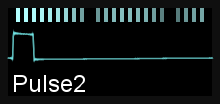
\includegraphics[scale=0.5]{6.png}\\
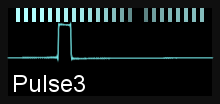
\includegraphics[scale=0.5]{7.png}
\vspace{-1em}
\end{wrapfigure}

Sometimes you need to customize the orientation in order to keep the zero position vertically centered. For example Blofeld's Arpeggiator has a variety of dials which aren't {\it quite} symmetric, because there are some unusual options at the start, as shown on the top figure at right.  But even worse: the Kawai K4 Effects patch has a number of dials which look like a {\it reversed} ``C'' because of so many additional options loaded at the end of the dial, as shown on the bottom figure.

\vspace{0.5em}You can customize the orientation in two ways.  First, if you override LabelledDial's {\bf isSymmetric()} method to return {\bf true}, then the dial will display itself as fully symmetric.  Second, you could override LabelledDial's {\bf getStartAngle()} method to return the desired angle of the start (leftmost) position of your curve.  The default is 270 (the ``C''), and when fully symmetric it's \mbox{90 + (270 / 2).}
\end{minipage}

\vspace{0.5em}When the user double-clicks on a LabelledDial, try to have the LabelledDial go to some default position.  This is often the ``zero'' position: but sometimes it's not.  At any rate, it's almost always most common position the user would want, whatever that is.  By default the ``default position'' is the first position if asymmetric, and the center position if symmetric.  You can change the default position by overriding LabelledDial's {\bf getDefaultValue()} method to return a different value.

Last but not least!  If you have a mixture of metric and non-metric values (for example, 0=``Off'', 1...32 = 1...32, and 33=``Uniform''), you will need to modify the MetricMin and MetricMax declarations.  Normally LabelledDial declares MetricMin to be the same as Min and MetricMax to be the same as Max.  But in this example, your minimum metric value is 1 and your maximum metric value is 32.

\begin{verbatim}
getModel().setMetricMin("whateverkey", 1);
getModel().setMetricMax("whateverkey", 32);
\end{verbatim}

It sometimes happens that {\it none} of the LabelledDial values should be thought of as metric.  For example, a previous code example, we were using the LabelledDial to select the MIDI Channel.  Now, channels aren't metric: they're just 16 unique labels for channels which happen to be numbers.  In this case, we should remove the metric min and max entirely, so Edisyn considers the entire range to be non-metric.  To do this, we say:

\begin{verbatim}
getModel().removeMetricMinMax("midichannel");
\end{verbatim}


\item {\bf IconDisplay}\quad This displays a different icon for each value in your model.  You can't change the values by clicking or dragging on an IconDisplay: instead, use a separate LabelledDial or Chooser.

\begin{verbatim}
ImageIcon icons = MY_ALGORITHM_ICONS;
JComponent comp = new IconDisplay("Algorithm Type", icons, this, "algorithmtype");
\end{verbatim}

Your images can be PNG or JPEG files: I suggest PNG.  You might create an instance variable like this:

\begin{verbatim}
public static final ImageIcon[] MY_ALGORITHM_ICONS = 
    {
    new ImageIcon(YamahaDX7.class.getResource("Algorithm1.png")),
    new ImageIcon(YamahaDX7.class.getResource("Algorithm2.png")),
    ... // and so on
    };
\end{verbatim}

These PNG files would be stored in your {\tt edisyn/synth/yamahadx7/} directory.


\item {\bf KeyDisplay}\quad This displays a keyboard.  You specify the min and max keys (which {\it must} be white keys), and a transposition (if any) between keys and the underlying MIDI notes actually generated.  When the user chooses a key, the KeyDisplay will update a value 0...127 corresponding to the equivalent MIDI note value.

The KeyDisplay can update {\it dynamically} or {\it statically}.  When dynamic, then every time you scroll through the display and a note is highlighted, the model is updated.  When static, the model is only updated when a note is finally chosen and the user has released the mouse button.  To set this, use {\bf setDynamicUpdate(...)}.  

You will probably want your KeyDisplay to update in concert with a LabelledDial.  This is easy: just set them to the same key in the model.  but synthesizers are inconsistent in how they describe notes, because MIDI didn't specify a notation.  For example, MIDI note 0 is ``C -2'' in Yamaha's notation (also adopted by Kawai and some others), or it is ``C -1'' in {\it Scientific Pitch Notation} (or SPN\footnote{... or {\it American Scientific Pitch Notation}(ASPN), or {\it International Pitch Notation} (IPN).  They're all pretentious names.}), or just play ``C 0'' in simple MIDI notation.  You can specify this by calling the method {\bf setOctavesBelowZero(...)}.

In some cases you might wish to be notified whenever the user {\it clicks} on a key, or drags to it, rather than when the key actually is updated (which might only happen on button release).  Typically this happens because you want to actually play the note so the user gets some feedback.  To be notified of this, just override the method {\bf userPressed(...)}.


\item {\bf PushButton}\quad This doesn't maintain a parameter at all: it's just a convenience cover for JButton.  You see it in Multimode patches where pressing it will pop up an equivalent Single patch (it's usually called ``Show''):

\begin{verbatim}
JComponent comp = new PushButton("Show")
    {
    public void perform()
        {
        // do your stuff here
        }
    };
\end{verbatim}

Popping up new synth panels from a multimode panel is complex.  Take a look at how {\tt edisyn/synth/waldorfmicrowavext/WaldorfMicrowaveXTMulti.java} does it.

\item {\bf EnvelopeDisplay}\quad This displays a wide variety of envelopes.  Envelopes are drawn as a series of points, and between every successive pair of points we draw a line.    You will provide the EnvelopeDisplay with several arrays defining the coordinates of those points.  

There are two main kinds of envelopes your synthesizer might employ.  First, your synthesizer might define parameters (like attack) in terms of the {\it height} of the attack and also the {\it amount of time} necessary to reach that height.  This is intuitive to draw, but in fact many synthesizers don't do it that way.  Instead, some define it in terms of the {\it height} of the attack and the {\it rate of change} (or slope, or angle).  In the first case, the height of the attack has no bearing on how long it takes to reach it.  But in the second case, the amount of time to reach the attack depends on both the height and on the rate.  This is even further complicated by some synthesizers (like Yamaha's) which use rate, but compute it not in terms of angle, but in terms of (essentially) 90 degrees {\it minus} the angle.  Thus a steeper rate is a {\it lower number}.  You will need to figure out what your synthesizer does exactly.  

Let's say your synth does the easy thing and computes stuff in terms of height and amount of time.  Then you set up an Envelope Display with four elements:

\begin{itemize}
\item An array of keys (some of which can be null) of the parameters which define the {\it amount of time} for each segment.  If a key is null, the parameter value is assumed to be 1.0.
\item An array of keys (some of which can be null) of the parameters which define the {\it height} for each segment.  If a key is null, the parameter value is assumed to be 1.0.
\item An array of constant doubles which will be multiplied against the time parameters.  You want these constants to be such that, when the time parameters are at their maximum length, their values, multiplied by these constants, will sum to  no more than 1.0
\item An array of constant doubles which will be multiplied against the height parameters.  You want these constants to be such that, when the any given height parameter is maximum, when multiplied against the constant it will be no more than 1.0.
\end{itemize}

Here's how you'd make an Envelope Display for an ADSR envelope where each of the values varies 0...127:

\begin{verbatim}
String[] timeKeys = new String[] { null, "attack", "decay", null, "release" };
String[] heightKeys = new String[] { null, "attackheight", "sustain", "sustain", null };
double[] timeConstants = new double[] { 0.0, 0.25 / 127, 0.25 / 127, 0.25, 0.25 / 127 };
double[] heightConstants = new double[] { 0.0, 1.0 / 127, 1.0 / 127, 1.0 / 127, 0.0 };
JComponent comp = new EnvelopeDisplay(this, Color.red, "ADSR", 
                timeKeys, heightKeys, timeConstants, heightConstants);
\end{verbatim}

Notice that {\tt "sustain"} is used twice: thus the line stays horizontal; and furthermore its time constant is fixed to 0.25 so it always takes up 1/4 of the envelope space.  Also notice that in this example the beginning and end of the ADSR envelope are fixed to 0.0 height.  That doesn't have to be the case.  And maybe you don't have an attack height: it's always full-on attack.  Then you'd say:

\begin{verbatim}
String[] heightKeys = new String[] { null, null, "sustain", "sustain", null };
double[] heightConstants = new double[] { 0.0, 1.0, 1.0 / 127, 1.0 / 127, 0.0 };
\end{verbatim}

It's possible that your envelope isn't always positive: it can go negative.   The EnvelopeDisplay normally assumes that your parameters are all positive numbers (like 0--127), but it does allow to draw a line indicating where the X axis should be, via the {\bf setAxis(...)} method.  See the fourth example in Figure \ref{envelopedisplays}.  You can also indicate that your Y values are {\it signed}, which means that when multiplied against their respective constants, they will range from -1...1 instead of from 0...1.  This is done with {\bf setSigned(...)}.

You also can also tell the EnvelopeDisplay to draw a vertical line at some key position and a dotted line at another, using the methods {\bf setFinalStageKey(...)} and {\bf setSustainStageKey(...)} respectively (these are named after their use in the Waldorf Microwave XT).  These keys should specify the {\it stage number} (the point) where the line is drawn.  For example, if the sustain stage key's value is 4, then the line should be drawn through point number 4 (zero-indexed) in the envelope.  See the third example in Figure \ref{envelopedisplays}.

You can also specify two intervals with start and stop keys respectively.  At present the EnvelopeDisplay supports two intervals.  These are set up with {\bf setLoopKeys(...)}.   These keys should specify the {\it stage number} (the point) where the intervals are marked.  For example, if the interval end's key value is 4, then the end should be marked exactly at point number 4 (zero-indexed) in the envelope.  Again, see the third example in Figure \ref{envelopedisplays}.

You can also postprocess the sustain stage, final stage, or loop keys with {\bf postProcessLoopOrStageKey(...)}.  This function takes a key and its value, and returns a revised value, perhaps to add or subtract 1 from it.

What if your synth uses angles/rates/slopes rather than time intervals?  For example, the Waldorf Blofeld does this. To handle this situation, we add an additional array of double constants called {\it angles}.   It works like this.  The height keys and height constants are exactly as before.  And {\tt timeConstants[0]} still defines the x position of the first point in the envelope, as before.  But the other time constants work differently.

Specifically, to compute the X coordinate of the next point, we take its key value and multiply it by the corresponding angle, and then take the absolute value.  This tells us the {\it positive angle} of the line.  Angles can never be negative: whether the line has a positive or negative slope is determined entirely by the relative position of the height keys.

Since angles can and will create very strung-out horizontal lines, the remaining time constants tell us the {\it maximum length} of a line: these again should sum to 1.0.

Angles/rates create weird idiosyncracies you'll have to think about.  For example, below is the code for the Blofeld's ADSR envelope.  As the Sustain gets higher, the Release gets longer but the Decay gets shorter, because the synth is basing this envelope on {\it rate} and not {\it time}.\footnote{Edisyn no longer displays this way for the Blofeld, because although the Blofeld indeed follows angle/rate, for large values the Blofeld's functions start getting close to following time.  The problem is that while the Blofeld documentation acknowledges that it follows angle/rate, the Blofeld's {\it screen} incorrectly displays envelopes following time!  When I wrote this documentation I was using angle/rate for the Blofeld because it's the ``true'' underlying behavior, but I've since changed the patch editor back to displaying time because using something other than what's on the Blofeld screen would really confuse owners, and in the Blofeld's case it's a subtle difference.}  One consequence of this is that the Decay and Release together are as long as the Attack, because if you're basing on rate, then the amount of time to go up is the same as the total amount of time to go {\it down}, and both Decay and Release go down.  Thus we have a {\it max width} of 1/3 for all four portions: but at any time they can only sum to 1/3 [attack] + 1/3 [sustain] + 1/3 [decay + release].

In the Blofeld ADSR, all the values go 0...127, and the angles are displayed by Edisyn to go from vertical to \(\pi/4\) (we don't want them too flattened out).  See if the code below makes sense now:

\begin{verbatim}
String[] timeKeys = new String[] { null, "attack", "decay", null, "release" };
String[] heightKeys = new String[] { null, null, "sustain", "sustain", null };
double[] timeConstants = new double[] { 0, 0.3333, 0.3333,  0.3333, 0.3333};
double[] heightConstants = new double[] { 0, 1.0, 1.0 / 127.0, 1.0/127.0, 0 };
double[] angles = new double[] { 0, (Math.PI/4/127),   (Math.PI/4/127), 0, (Math.PI/4/127) };
JComponent comp = new EnvelopeDisplay(this, Color.red, "ADSR", 
                timeKeys, heightKeys, timeConstants, heightConstants, angles);
\end{verbatim}

Sometimes you need {\it both} angles {\it and} times.  For example, in the E-Mu Ultra Proteus, attack and decay and release are measured in rate, but ``hold'' measures how long (in time) we stay at maximum attack before starting decay.  To do this, if you set the appropriate angle to {\tt EnvelopeDisplay.TIME}, then the corresponding time constant will revert to being used as a measure of time rather than a maximum length for the angle.

This {\it still} might not be flexible enough for you.  For example, the Yamaha TX81Z has, shall we say, an unusual approach to defining angles.  You can do further post processing on the \(\langle x,y\rangle\) coordinates of each of the points (where  both X and Y vary from 0...1) by overriding the {\bf postProcess(...)} method like this:

\begin{verbatim}
JComponent comp = new EnvelopeDisplay(this, Color.red, "ADSR", 
                timeKeys, heightKeys, timeConstants, heightConstants, angles)
    {
    public void postProcess(double[] xVals, double[] yVals)
        {
        // modify xVals and yVals as you see fit.
        }
    };
\end{verbatim}

Envelopes generally stretch to fill all available space: they're particularly good to put as the ``last'' element in an HBox via addLast().  But you might want to add them elsewhere and fix them to a specific width. In this case, just call {\bf setPreferredWidth(...)}.

\item {\bf Other Objects}.  There are other custom widgets strewn throughout Edisyn, including number-entry fields (see the MicroKorg), Joysticks (see the Wavestation SR), cross-fade envelopes (Wavestation SR again), and much more complex versions of envelope displays for things like harmonics or filters (see the Kawai K5 and the FS1R Fseq).  

\end{itemize}

\paragraph{Spacing and Positioning}

Edisyn handles most positioning using VBox, HBox, and JPanels set to BorderLayout.  However there are some cases where this is not sufficient to push objects to the right spot.  To this end, Edisyn also provides:

\begin{itemize}
\item {\bf Strut}.  This is a fixed blank space of zero height and non-zero width, or the other way around.  It's useful to add to an HBox or VBox to push an object to a certain position.  You can also make a Strut that is the exact same dimensions of an existing object.  For example, imagine if you wanted a row of dials, and below it a second row of dials, but with one dial missing (but with the gap left).  You could put a Strut there, set to the size of the LabelledDial above it.

\item {\bf Stretch}.  This is a blank space which stretches to consume all available space in its box, pushing everything else out of the way.
\end{itemize}

\paragraph{Dynamically Changing Widgets}

One gotcha which shows up in a number of synthesizers (particularly in effects sections) is that if you change (say) the effect type, the number of available parameters, and their names, will change as well.  Eventually Edisyn will have a widget that assists in this, but for now you'll have to manually add and remove widgets.

Edisyn's patch editors usually do this by defining a bunch of HBoxes, one for each effect type, and then remove the current HBox and add the correct new one dynamically in response to the user changing types.  You can see a simple example of this in the Waldorf Microwave XT code, and a more elaborate version in the Blofeld code (where different effects actually share specific widgets).  This is often triggered inside the {\tt update} method of a Chooser (for the effect type, say).

You'll have to manually remove and add these widgets or HBoxes.  But when should you do so?  That's pretty easy: when the effect type has been updated.  Typically the effect type is shown as a Chooser, and when it is updated, the Chooser's {\bf update(...)} method is called:

\begin{verbatim}
JComponent comp = new Chooser("Effect Type", this, "effecttype", types)
    {
    public void update(String key, Model model)
        {
        super.update(key, model);  // be sure to do this first
        int newValue = model.get(key, 0);  // 0 is the default if the key doesn't exist, but it will.
        
        // now do something according to the value newValue
        }
    };
\end{verbatim}

You'll see various patch editors have implemented update(...) for various purposes.

Hand in hand with this: in some rare cases you want the update(...) method to be called not only when the widget's key is updated, but when {\it some other key} is updated.  To do this, you can {\it register} a widget to be updated for that key as well.  This is done as follows:

\begin{verbatim}
model.register("keyname", widget);
\end{verbatim}

For example, in the Yamaha TX81Z, the operator frequency is computed as a combination of three widgets: and in the final widget (``Fine'') the final frequency is displayed.  To do this, we have registered the ``Fine'' widget to revise itself (via the map(...) method) whenever any of three different parameters is updated.

\subsection{Getting Input from the Synth (and File Loading) Working}
\label{filereading}

There are three common ways the synth can send you information: as a sysex patch dump, as a bank sysex message, and as individual parameters.  We'll start with the sysex patch dump.

\paragraph{Recognizing Sysex and Parsing Patch Dumps}
Let's start by setting up our recognizer, which is stored in the {\tt edisyn/synth/yamahadx7/YamahaDX7Rec.java} file.  This file contains code which recognizes whether incoming sysex messages should be routed to the DX7, among other tasks.  \footnote{You'll note that each synthesizer file has an accompanying recognizer file.  Why not just put the recognizer methods in the synthesizer class?  There's a good reason.  When Edisyn encounters a sysex message, it must go through {\it all} of the synthesizers and ask them one by one if they recognize the message and are capable of parsing it.  To do this would require that Edisyn load all of the class files for the synthesizers: and some class files are {\it enormous}, with huge numbers of strings and other tables.  Check out the Yamaha FX1R patch code for example!  So instead Edisyn just goes though all the recognizer classes instead, which are very small classes and can be checked very rapidly.  Only when it knows it has a sysex message for a given synthesizer does it actually load its class and instantiate it.}   Give it the proper class name and package.

Next, we need to implement the {\bf recognize(...)} method in our recognizer file.  This method tells Edisyn that you recognize a dump sysex message.  You should verify the message length and the header to determine that it's a patch dump and in fact meant is for your type of synthesizer {\it and} is probably correct.  This method will also be called when loading a sysex file from disk.  Here's a simple recognizer for the DX7:

\begin{verbatim}
    public static boolean recognize(byte[] data)
        {
        return ((data.length == 163 &&
                data[0] == (byte)0xF0 &&
                data[1] == (byte)0x43 &&
                // don't care about 2, it's the channel
                data[3] == (byte)0x00 &&
                data[4] == (byte)0x01 &&
                data[5] == (byte)0x1B));            
        }
\end{verbatim}

Next, you need to implement the {\bf parse(...)} method in the main {\tt YamahaDX7.java} file.  In this method you will be given a byte array and your job is to set the model parameters according to your parsing of this array.  You set parameters using the {\bf set(...)} methods in the model, like this:

\begin{verbatim}
getModel().set(numericalKey, 4.2);		// or whatever new value
getModel().set(stringKey, "newValue");	// or whatever new value
\end{verbatim}

If the parse was successful, you should usually return {\tt PATCH\_SUCCEEDED}.  If you queried the user for more information (Synth.java has good query dialog box methods for you) and the user cancelled the parsing, you should return {\tt PATCH\_CANCELLED}.  If the parse failed due to corruption, say, return {\tt PATCH\_FAILED}.

\paragraph{Recognizing and Parsing Multi-Sysex Patch Dumps}
Most synthesizers are sane and have one sysex message per patch.  But some are not.  For example, the Yamaha 4-op FM family have patches which consist of up to {\it four} messages in a row!  How is this handled?

The first issue lies in {\bf bulk patch files}.  A bulk patch file is a file which contains multiple individual patches, possibly from different kinds of synthesizers, or at least different kinds of patches for the same synth, such as single matches versus multimode patches versus, um, effect patches.  In a perfect world, if the file contained \(N\) patches, it'd contain \(N\) sysex messages concatenated together.  Unfortunately since some synths have multiple sysex message per patch, this can get very complicated.   Edisyn needs to know what messages form a patch, because some files can have some \(M\) of these messages concatenated together to form some \(N<M\) patches altogether.   

If your synth requires multiple messages for a single patch, you need you recognizer to implement this method:

\begin{verbatim}
    public static int getNextSysexPatchGroup(byte[][] sysex, int start);
\end{verbatim}

This method is given an array of sysex messages and a {\it start} position.  Beginning with the message {\tt sysex[start]} is a patch, possibly consisting of multiple messages, which your synthesizer might or not might not recognize.  If the patch is not for you, return {\tt start}.  Otherwise, let's say you have determined that the patch consists of the next three messages.  Then you should return {\tt start + 3}.  If your synth always uses one message per patch, don't bother implementing this method.

The second issue lies in {\bf incomplete patch dumps}.  When you receive a dump through parse() via the synth over MIDI, it'll likely contain exactly one sysex message.  Thus if your patch requires multiple sysex messages, parse() will be ultimately called several times before you've gotten an entire patch.  However when you receive a dump via a file, the data will likely contain {\it all} of these messages.  Thankfully, the parse() method will tell you whether you're receiving from a file or not.  

At any rate, if you have yet not received all of the messages necessary to completely parse the patch, you should parse what you can, then return {\tt PATCH\_INCOMPLETE}.  In all likelihood parse() will be called later with the remaining information.

\paragraph{Recognizing and Parsing Bank Sysex Dumps}

Some synthesizers can send entire banks of patches as a single sysex message.  The Yamaha DX7 can do this, for example, and in fact it's the standard way DX7 patches are stored on the internet.

To handle bank sysex dumps, you need to first recognize them.  In {\tt YamahaDX7Rec.java}, you need to implement the {\bf recognizeBulk(...)} method.  This method should work just like recognize(), except that it recognizes bank sysex messages.  Here's a simple DX7 Bulk recognizer method:

\begin{verbatim}
    public static boolean recognizeBulk(byte[] data)
        {
        return  (data.length == 4104 &&
            data[0] == (byte)0xF0 &&
            data[1] == (byte)0x43 &&
            // don't care about 2, it's the channel
            data[3] == (byte)0x09 &&
            // data[4] == (byte)0x20 &&          // sometimes this is 0x10 by mistake
            data[5] == (byte)0x00);
        } 
\end{verbatim}

Next you need to modify recognize() so that if recognizeBulk() returns true, then recognize() does also.  This is easily done by having recognize call recognizeBulk() internally, such as:

\begin{verbatim}
    public static boolean recognize(byte[] data)
        {
        return (
            // 1 single
                (data.length == 163 &&
                data[0] == (byte)0xF0 &&
                data[1] == (byte)0x43 &&
                // don't care about 2, it's the channel
                data[3] == (byte)0x00 &&
                data[4] == (byte)0x01 &&
                data[5] == (byte)0x1B) 
            // bulk
            || recognizeBulk(data));
        }
\end{verbatim}

Next, you need to modify the {\bf parse(...)} method in the main {\tt YamahaDX7.java} file so that it handles bank sysex messages.  In Edisyn this is done by querying the user as to which patch he wishes to edit from that sysex message (or whether he'd like to do other operations, such as upload the entire bank sysex to the synthesizer, or save it as a file).  

This is done by first extracting the names from the bank sysex message received in parse().  With the names in hand, call {\bf showBankSysexOptions(...)}, passing in the data and the names.  The method will then return either the patch the user has selected, or a negative value indicating that no parse should be done.  If the user has selected a patch, parse it from the bank sysex.

\paragraph{Requesting a Patch from the Synthesizer}

In order for the user to request a patch from the synthesizer, he needs to be able to specify the bank and number.  To do this, you need to implement the {\bf gatherPatchInfo(...)} method.   This method is used for both requesting patches and for writing them: on many synths certain banks are read-only, so they should vary depending on whether requesting or writing is being performed.

This method is nontrivial to implement. I suggest you take a look at existing patch editors to see how they have implemented it, and largely copy that.  You'll notice that patch-gathering code usually pops up a dialog box with a bunch of rows in it.  How is this done?  Edisyn's Synth.java class has a special method to make this easy: {\bf showMultiOption(...)}. 

Next you need to override methods which issue a dump request to the synth:

\begin{itemize}
\item {\bf performRequestDump(...)} or {\bf requestDump(...)}\quad Override {\it one} of these methods to request a dump from the synth of a specific patch.  requestDump(...) is simpler: you just return bytes corresponding to a sysex message to broadcast to the synth.  performRequestDump(...) lets you manually issue the proper commands. 

In the second case, the edisyn.Midi class, instantiated in the {\bf midi} instance variable, has several methods for constructing MIDI messages: you can send them, or send sysex messages (as byte arrays) via the {\bf tryToSendMIDI()} or {\bf tryToSendSysex()} methods.  Also you'll have to handle changing the patch: see the information in Blank.java's documentation on this method for an example.

Both of these methods take a Model called {\bf tempModel} which will hold information concerning the patch number and bank number that you should fetch.  This model was built by gatherPatchInfo(...).

\item {\bf performRequestCurrentDump(...)} or {\bf requestCurrentDump(...)}\quad Override {\it one} of these methods to request a dump from the synth of the current patch being played.  These methods are basically just like performRequestDump(...) and requestDump(...), but they don't take a model (there's no patch number).
\end{itemize}

Finally, you will also probably need to implement {\bf changePatch(...)} to issue a patch change (it'll be called as part of performRequestDump(...)).    It's possible that your synthesizer must pause for a bit after a patch change (the Blofeld, for example, requires almost 200ms).  You may want to implement the {\bf getPauseAfterChangePatch()} method to slow Edisyn down.  If your synth can't change patches to whatever you're editing, that's okay, but you'll need to handle the right behavior later on when you emit a patch to it.

Patch requests often are complicated:

\begin{itemize}
\item Some synthesizers dump patches from patch memory but do not automatically put them into current working memory.  Others do.  This probably won't matter because Edisyn will update the current working memory when the patch is received. 
\item Some synthesizers do not include the patch bank and number in their patch dumps.  Thus you will have to call changePatch(...) from within requestDump(...) to preemptively update Edisyn's belief about the current patch in anticipation of the patch coming in.
\item Some synthesizers cannot dump patches from patch memory at all: you have to ask them to load the patch into current working memory, and then request a dump of current working memory.  This would have to be done inside requestDump(...), commonly as a request to move the patch to current working memory, and then a call to requestCurrentDump(...).
\item Some synthesizers cannot dump patches from current working memory at all.  If your synth cannot dump the current patch you can avoid implementing some of these methods by saying the following:

\begin{verbatim}
receiveCurrent.setEnabled(false);  // turns of the "Request Current Patch" menu option
\end{verbatim}

You should do this in an overridden version of the  {\bf sprout()} method (be absolutely certain to call \mbox{super.sprout()} first).
\item There are more weird gotchas than just these\,---\,you might peruse Edisyn's existing editors for strategies to deal with them.
\end{itemize}

You will also want to override some other methods.  First {\bf getPatchName(model)} should extract the patch name from the provided model (probably via {\tt model.get("name", "foo")}\ ).  Second, you also will want to override the {\bf revisePatchName(...)} method if you've not already done so for the StringComponent widget.  This method modifies a provided name and returns a corrected version.  The default version, which you might call first (via super), removes trailing whitespace.  You can then revise incorrect characters, length, and so on.  Third, if your synthesizer uses an ID to distinguish itself from other synthesizers of the same type (the Waldorf synths do this for example), you should override the {\bf reviseID(...)} method to correct provided IDs.  If this method returns {\tt null} (the default), the  ID won't even appear as an option.

Finally, you will probably want to override the {\bf revise()} method to verify that all the model parameters have valid values, and tweak them if not.  The default version, which you can call via super, does most of the heavy lifting: it bounds the values to between their min and max.  You might also verify that the patch name is correct here.  See the Waldorf Blofeld code as an example of what to do.

See also the description of these methods in {\tt edisyn/synth/Blank.java}

\paragraph{Individual Parameters}

{\it [If your synth doesn't send out individual parameters, or you don't want to be bothered right now in handling this, you can just ignore this section for now].}

Individual parameters might come in as sysex messages, as CC messages, or as NRPN.  Here are your options:

\begin{itemize}
\item {\bf Sysex Messages}\quad Here, override the method {\bf parseParameter(...)}.  Note that the provided data might be something else sent via sysex besides just a parameter change.  You can test for that too (and handle it here if you like).  Also, your recognizer should {\it not} recognize individual parameter messages, or else they'll be sent to parse() rather than parseParameter().  You don't want that.

\item {\bf NRPN or Cooked CC messages}\quad A cooked CC message is one which doesn't violate any of the RPN/NRPN rules (it's not 6, 38, 97, 98, 99, 100, or 101).  At present Edisyn does not recognize 14-bit CC.  If your messages are always cooked or are NRPN, then you can handle them via {\bf handleSynthCCOrNRPN(...)}, which takes a special {\bf MIDI.CCData} argument that tells you about the message (see the Midi.java class). 

\item {\bf Raw CC Messages}\quad A raw CC message is any message number 0...127 just sent out willy-nilly, not respecting things like RPN/NRPN or 14-bit CC.  If your synth sends out raw CC messages, you need to override {\bf getExpectsRawCCFromSynth()} to return {\bf true}.  Then you handle the messages via  {\bf handleSynthCCOrNRPN(...)} as discussed above.
\end{itemize}

Again, you update one or more parameters in response to these messages using one of:

\begin{verbatim}
getModel().set(numericalKey, 4.2);		// or whatever new value
getModel().set(stringKey, "newValue");	// or whatever new value
\end{verbatim}

\paragraph{Note on File Loading}

If your patch dumps come in as sysex messages, then congratulations, you already have file loading working.  If not, you will need to {\it invent} a patch sysex format and implement it in the {\bf parse(...)} (and later {\bf emit(...)} methods even if your synthesizer never sends stuff via sysex (such as is the case in the PreenFM2).  That way you can still load and save files.  

You probably ought to use the ``educational use'' wildcard MIDI sysex ID (0x7D).  Edisyn's made-up sysex header for the PreenFM2 currently looks like this: {\tt 0xF0, 0x7D, 'P', 'R', 'E', 'E', 'N', 'F', 'M', '2', {\it version}.}  Presently {\it version}  is {\tt 0x0}.  You might do something similar.

\subsection{Getting Output to the Synth (and File Writing) Working}

If you've gotten this far, writing is simpler than parsing and requesting, because you've already written a lot of the support code.  You can write out both patch dumps and individual parameters (as you tweak widgets).

\paragraph{Patch Dumps}

You will need to implement {\it one} of the following two methods: either {\bf emitAll(Model, ...)} or {\bf emit(Model, ...)}.  The emit(Model, ...) method is simpler: you just build data for a sysex message and return it.  In emitAll(Model, ...), you build an array consisting of {\it either} javax.sound.midi.SimpleMessage objects {\it or} byte[] arrays corresponding to sysex messages, or a mixture of the two.  These will be emitted one by one.  Most commonly you just override emit(Model, ...).

Both emit(Model, ...) and emitAll(Model, ...) receive a temporary model.  This model will contain a small bit of data sufficient to inform you of the patch and bank number are that the patch is going to be emitted to (via Edisyn's ``write'' procedure).  Alternatively if the {\it toWorkingMemory} argument is TRUE, then you're supposed to emit to current working memory (Edisyn's ``send'' procedure).

You may not be able to write, or you may not be able to send to a specific patch, or to the current patch, depending on your synthesizer.  If so, you can do any of:

\begin{verbatim}
%transmitTo.setEnabled(false);  // turns of the "Send to Patch..." menu option
transmitCurrent.setEnabled(false);  // turns of the "Send to Current Patch" menu option
writeTo.setEnabled(false);  // turns of the "Write to Patch..." menu option
\end{verbatim}

Again, these should be set in an overridden version of the {\bf sprout()} method.  Be sure to call {\bf super.sprout()} first, or bad things will probably happen.

Note that emit(Model, ...) and emitAll(Model, ...) are also used to write out files.  If you implemented emitAll(...), be aware that Edisyn will strip out all of the javax.sound.midi.SimpleMessage messages and just pack together then remaining sysex messages.  This is what will result in multiple sysex messages being read in in a single parse(...) dump, as discussed earlier.  

Some synthesizers need a bit of time to rest after receiving a dump before they can do anything else.  You can tell Edisyn to pause after a dump by overriding {\bf getPauseAfterSendAllParameters()}.

\paragraph{Individual Parameters}

In response to changing a widget, Edisyn will try to change a parameter on your synthesizer.  This is similar to the patch dump.  Specifically, there are two methods, {\bf emit(String)} and {\bf emitAll(String)}, which work like their patch counterparts, except that they are tasked to emit a {\it single parameter} to the synthesizer.  Implement only {\it one} of these methods.  If you don't want to do this, just don't implement these methods.

If your synthesizer accepts NRPN (such as the PreenFM2), the Midi.java file has some utility methods for building NRPN messages easily.

It's possible that your synthesizer can only accept messages at a certain rate.  You may want to implement the {\bf getPauseBetweenMIDISends()} method to slow Edisyn down.

\paragraph{Patch Dumps Via Individual Parameters}

Some synthesizers, such as the PreenFM2, do not accept a patch dump method at all.  Rather you send a ``patch dump'' as a whole lot of individual parameter changes.  If your synthesizer is of this type, you should override the method {\bf getSendsAllParametersInBulk()} method to return {\bf false}.

\paragraph{Note on File Writing}

See the earlier note at the end of Section \ref{filereading} about File Loading: as discussed there, if your synth doesn't read or write sysex, you'll still need to {\it invent} a patch sysex format, and implement it in the {\bf emit(...)} and {\bf parse(...)} methods, so you can save and load files to disk.


\subsection{Creating an Init File}

Now that you've got everything coded and working (hah!) it's time to create an Init file.  To do this, either request an init patch from the synthesizer, or create an appropriate one yourself.  Then save it out as a sysex file.

Next, move that file and rename it to {\tt edisyn/synth/yamahadx7/YamahaDX7.init}.  Edisyn will load this file to initialize your patch editor.  To do this, add to the very bottom of your constructor the following line:

\begin{verbatim}
loadDefaults();
\end{verbatim}

\subsection{Getting Batch Downloads Working}

Edisyn can download many patches at once.  To support this, you need to implement a few methods.\footnote{Until you implement {\bf getPatchLocationName(...)} to return something other than {\tt null}, Edisyn will keep the Batch Downloads menu disabled.  So when you implement this method, be sure to also implement the other methods here at the same time.} First, there's {\bf getPatchLocationName(...)}, which returns as a String a short version of the patch address (bank, name) to be used in a saved filename.  Next, there's {\bf getNextPatchLocation(...)} which, given a Model containing a patch address, returns a model with the ``next'' patch address (wrapping around to the very first address if necessary).  Finally you need to implement {\bf patchLocationEquals(...)}, which compares two patches to see if they contain the same patch address.
 
A few synthesizers (notably the PreenFM2) don't send individual patches as single sysex patch dumps, but rather send them as multiple separate NRPN or CC messages.  Edisyn needs to know this so it can make a better guess at whether a patch dump has arrived and is ready to be saved.  To let Edisyn know that your patch editor is for a synthesizer of this type, override the method {\bf getReceivesPatchesInBulk()} to return false.

Compared to the other stuff, this step is easy.\footnote{Note that lots of synthesizers have sysex facilities to dump the entire patch memory, or dump an entire bank, etc.  Edisyn doesn't use these; it requests patches one by one.  This is slower but saves you a lot of coding and is consistent across synthesizers.  So you're welcome.}

\subsection{Building the Librarian}

Getting the Librarian working largely involves implementing certain hook functions.  

\paragraph{Bank Layout}

First you need to define the bank structure of the synthesizer.  This can be as simple as a single bank, or as complex as dynamically-changing banks of different sizes and structures (see the nightmare that is the Proteus 2000).  Implement {\bf getBankNames()} to indicate the names of the banks, unless you have only one bank, and {\bf getWriteableBanks()} to indicate which banks are read/write and which are read-only (you might use the utility method {\bf buildBankBooleans()} to help out).  The names of the patch locations are stated via {\bf getPatchNumberNames()} (you might use the utility method {\bf buildIntegerNames()} to help out).  

Edisyn uses {\bf getBankNames()} to determine the number of banks, and {\bf getPatchNumberNames()} to determine the typical number of patches per bank (and if {\bf getPatchNumberNames()} returns null, Edisyn doesn't provide a Librarian at all).  But some banks may vary in size relative to one another or have certain invalid patch number locations compared to other banks.  Others have banks that are appropriate only in some circumstances (such as when a certain card is installed).  You can specify this via {\bf isValidPatchLocation(...)}, {\bf isAppropriatePatchLocation(...)}, and possibly {\bf getValidBankSize(...)}.

You specify the size of a cell with {\bf getPatchNameLength()}.  Some rare synthesizers (notably the Yamaha FB-01) allow you to change the name of a bank in addition to a patch.  This is done with {\bf reviseBankName(...)}.

\paragraph{Individual Patch Sysex versus Bank Sysex}  Generally speaking there are three kinds of synthesizers:

\begin{itemize}
\item Ones that read and write individual patches (the Oberheim Matrix 1000 for example)
\item Ones that can only read and write whole banks at a time (the Yamaha DX7 for example)
\item Ones that can read and write both individual patches and whole banks (the Kawai K4 for example).  In this case Edisyn will request both banks and individual patches, but typically will only write individual patches to keep things simple.  
\item Ones that can't use a librarian at all (the MicroSampler for example).
\end{itemize}

You can indicate which of the above types your synthesizer is by overriding the {\bf getSupportsDownloads()}, {\bf getSupportsPatchWrites()}, {\bf getSupportsBankReads()}, and {\bf getSupportsBankWrites()} methods.  

If your synthesizer only supports individual patch request and writes, this may be all you need to do (other than {\bf librarianTested()} below).  But if your synthesizer deals with whole banks at a time, you will need to override some additional methods.

First, you'll need to determine which bank a given sysex message represents, with {\bf getBank(...)} or (if need be {\bf getBanks(...)}).  Next, you need to be able to extract and parse an individual patch from a bank sysex message with {\bf parseFromBank(...)}, to convert a bank of models into a bank-sysex message with {\bf emitBank(...)}, and to specify the pause afterwards with {\bf getPauseAfterWriteBank()}.  Edisyn will need to know how to request a bank (as opposed to an individual patch).  This is done with {\bf requestBankDump(...)}.  Some synthesizers have a bank-request message only for a single bank (the others must be requested per-patch): you can specify this with {\bf getRequestableBank()}. 

\paragraph{Final Touches}

Certain synthesizers have special sysex messages which trigger them to dump all their patches rapidly. You can provide this sysex with {\bf requestAllDump()}.  Others have a special sysex message to request the dump of an individual bank.  This can be triggered with {\bf requestBankDump(...)}.

Very large patch editors are slow and costly, and may have memory leaks, if you update their listeners on downloading a patch into a Librarian.  You can prevent this by overriding {\bf getUpdatesListenersOnDownload}.

Once you've verified your librarian works, override {\bf librarianTested()}.

\subsection{Other Stuff}
You're almost done!  Some other items you might want to do.  First, you may need to tweak the mutability of parameters.  No string parameters are mutable, but by default all numerical ones are (including checkboxes and choosers).  Occasionally you'd want to make some of those immutable so they will not be modified during merge, hill-climbing, etc.  To do this, you can call {\bf setStatus(..., Model.STATUS\_IMMUTABLE)} on the model.

Second, whenever your patch editor becomes the front window, the method {\bf windowBecameFront()} will be called.  You could override this to send a special message to your synth to update it somehow.  For example, the Waldorf Microwave XT patch editors send a message to the Microwave XT to tell it to switch from single to multi-mode (or back) as appropriate.

Third, when the user clicks on the close box, the method {\bf requestCloseWindow()} is called.  You can override this to query the user about saving the patch etc. first, and then finally return the appropriate value to inform Edisyn that the window should in fact be closed.  Though in fact currently no patch editors implement this method at all.

There are many more methods available in {\tt Synth.java} which customize how long it pauses in different situations, how it sends and receives information, etc.  You may need to implement these as necessary.  See {\tt Blank.java} for explanations and default implementations of many of these methods.

\subsection{Submitting Your Patch Editor!}

\begin{itemize}
\item Clean up the editor code, make it really polished, well documented, and good looking.
\item Test it well (see below).
\item Copyright your editor code at the top of the file.  License the editor code under Apache 2.0 (I don't accept anything else).
\item Send the whole directory to me!  I'd love to include it.
\end{itemize}

\vbox
{
\paragraph{Some Testing Resources}
\begin{itemize}
\item Make sure you have tools for examining files and watching the MIDI device. I develop on the Mac, so make extensive use of {\tt hexdump} to examine sysex files, as well as the enormously valuable {\tt MIDI Monitor} to spy on sysex and other messages as they come and go.
\item You can sanity-check your patch editor with {\tt java edisyn.test.SanityCheck -h} which will build an instance of your synth, randomize it, write it to a stream, read it in from the same stream again, and compare the two models to see if they're the same.  In some cases the models {\it cannot} be the same and that's okay: in this case it will call {\tt testVerify(...)} on your synth class with the problematic keys in question, and if you return true, it'll ignore those keys.  Otherwise it'll report an error.
\item There is a static final variable called {\tt Model.debug}.  If you set it to true, then all reads and writes to the model are logged so you can watch them happening.
\item There is a static final variable called {\tt Style.showRaw}.  If you set it to true, then both the Choosers and LabelledDials will show the actual integer values of their underlying model parameters rather than (or in addition to) their mapped Strings.
\item {\tt StringUtility.toHex(...)} is useful for printing things out, as is {\tt Synth.printSysex(...)}.
\item The method {\tt edisyn.util.SyxSplit.main(...)} can be run run with a sysex file as its sole argument. It will split the file into separate files, one per sysex message in the original file.
\end{itemize}
}

\end{document}
